\chapter{Systematic uncertainty}
\label{ch:sys-unc}

\section{Experimental systematics}

\begin{table}[h]
    \scriptsize
    \begin{center}
        \begin{tabular}{ll}
            \hline
            \hline
            Systematic uncertainty & Short description \\
            \hline
            \multicolumn{2}{c}{\textbf{Event}} \\
            \hline
            Luminosity & Uncertainty on the total integrated luminosity \\
            \hline
            \multicolumn{2}{c}{\textbf{Electrons}} \\
            \hline
            EL\_EFF\_Trigger\_TOTAL\_1NPCOR\_PLUS\_UNCOR & Trigger efficiency uncertainty \\
            EL\_EFF\_Reco\_TOTAL\_1NPCOR\_PLUS\_UNCOR & Reconstruction efficiency uncertainty \\
            EL\_EFF\_ID\_TOTAL\_1NPCOR\_PLUS\_UNCOR & ID efficiency uncertainty \\
            EL\_EFF\_Iso\_TOTAL\_1NPCOR\_PLUS\_UNCOR & Isolation efficiency uncertainty \\
            EG\_SCALE\_ALL & Energy scale uncertainty \\
            EG\_RESOLUTION\_ALL & Energy resolution uncertainty \\
            \hline
            \multicolumn{2}{c}{\textbf{Muons}} \\
            \hline
            mu20\_iloose\_L1MU15\_OR\_HLT\_mu40\_MUON\_EFF\_Trig & Trigger efficiency uncertainties \\ 
			mu24\_ivarmed\_OR\_HLT\_mu40\_MU\_EFF\_TrigStat & None \\ 
			mu24\_ivarmed\_OR\_HLT\_mu50\_MU\_EFF\_TrigStat & None \\ 
			mu26\_ivarmed\_OR\_HLT\_mu50\_MU\_EFF\_TrigStat & None \\ 
            MUON\_EFF\_RECO\_STAT & Reconstruction uncertainty for \pt $>15GeV$ \\
            MUON\_EFF\_RECO\_SYS & None \\ 
			MUON\_EFF\_RECO\_STAT\_LOWPT & \speciallcell{Reconstruction and \\ID efficiency uncertainty for \pt $<15GeV$} \\ 
			MUON\_EFF\_RECO\_SYS\_LOWPT & None \\ 
			MUON\_ISO\_STAT & Isolation efficiency uncertainty \\ 
			MUON\_ISO\_SYS & None \\ 
			MUON\_TTVA\_STAT & Track-to-vertex association efficiency uncertainty \\ 
			MUON\_TTVA\_SYS & None \\ 
            MUONS\_SCALE & Energy scale uncertainty \\
            MUONS\_SAGITTA\_RHO & Variations in the scale of the momentum \\
            MUONS\_SAGITTA\_RESBIAS & Variations in the scale of the momentum \\
            MUONS\_ID & Energy resolution uncertainty from inner detector \\
            MUONS\_MS & Energy resolution uncertainty from muon system \\
            \hline
            \multicolumn{2}{c}{\textbf{\met-Trigger and \met-Terms}} \\
            \hline
            METTrigStat & Trigger efficiency uncertainty \\
            METTrigSyst & None \\
            MET\_SoftTrk\_ResoPerp & \speciallcell{Track-based soft term related to \\transversal resolution uncertainty} \\ 
			MET\_SoftTrk\_ResoPara & \speciallcell{Track-based soft term related to \\longitudinal resolution uncertainty} \\
			MET\_SoftTrk\_Scale & \speciallcell{Track-based soft term related to \\longitudinal scale uncertainty} \\
			MET\_JetTrk\_Scale  & \speciallcell{Track \met scale uncertainty \\due to tracks in jets} \\
            PRW\_DATASF & \speciallcell{Uncertainty on data SF used \\for the computation of pileup reweighting} \\
            \hline
            \hline
		\end{tabular}
	\end{center}
	\caption{A summary of the experimental systematic uncertainties.}
	\label{tab:c8:expsyst1}
\end{table}

\begin{table}[h]
    \scriptsize
    \begin{center}
        \begin{tabular}{ll}
            \hline
            \hline
            Systematic uncertainty & Short description \\
            \hline
            \multicolumn{2}{c}{\textbf{Small-radius jets}} \\
            \hline
            JET\_EtaIntercalibration\_Modelling & $\eta$-intercalibration: MC generator modelling uncertainty \\
            JET\_EtaIntercalibration\_TotalStat & $\eta$-intercalibration: statistical uncertainty \\
            JET\_EtaIntercalibration\_NonClosure\_highE & \speciallcell{$\eta$-intercalibration: non-closure uncertainty \\of jet response, high energy component} \\
            JET\_EtaIntercalibration\_NonClosure\_negEta & \speciallcell{$\eta$-intercalibration: non-closure uncertainty \\of jet response, negative $\eta$ component} \\
            JET\_EtaIntercalibration\_NonClosure\_posEta & \speciallcell{$\eta$-intercalibration: non-closure uncertainty \\of jet response, positive $\eta$ component} \\
            JET\_Pileup\_OffsetMu & Pileup: Offset, term for number of interactions per crossing $\mu$ \\
            JET\_Pileup\_OffsetNPV & Pileup: Offset, term for number of primary vertices \\
            JET\_Pileup\_PtTerm & Pileup: Offset, \pt term \\
            JET\_Pileup\_RhoTopology & Pileup: Offset, $\rho$ topology uncertainty on jet areas \\
            JET\_Flavor\_Composition & Flavor composition uncertainty \\
            JET\_Flavor\_Response &  Flavor response uncertainty (dominated by gluon response) \\
            JET\_PunchThrough\_MC16 & Punch-through correction uncertainty \\
            JET\_EffectiveNP\_Statistical & \speciallcell{Statistical components of effective jet energy scale uncertainties, \\split into 6 components} \\
            JET\_EffectiveNP\_Modelling & \speciallcell{Modelling components of effective jet energy scale uncertainties, \\split into 4 components} \\
            JET\_EffectiveNP\_Detector & \speciallcell{Detector components of effective jet energy scale uncertainties, \\split into 2 components} \\
            JET\_EffectiveNP\_Mixed & \speciallcell{Effective jet energy scale uncertainties coming from various sources, \\split into 3 components} \\
            JET\_SingleParticle\_HighPt & Uncertainty related to high \pt jets \\
            JET\_RelativeNonClosure\_MC16 & Closure of the calibration, relative to MC12a \\
            JET\_BJES\_Response & Jet energy scale uncertainty for $b$-jets \\
            JET\_JER\_DataVsMC\_MC16 & \speciallcell{Nuisance parameter covering when jet energy resolution \\in data smaller than resolution in MC} \\
            JET\_JER\_EffectiveNP & Effective jet energy resolution uncertainty; split into 6 components \\
            FT\_EFF\_EIGEN\_B & $b$-tagging efficiency uncertainties ("BTAG\_MEDIUM) \\
            FT\_EFF\_EIGEN\_C & None \\
            FT\_EFF\_EIGEN\_L & None \\
            FT\_EFF\_EIGEN\_extrapolation & $b$-tagging efficiency uncertainty on the extrapolation on high \pt-jets \\
            FT\_EFF\_EIGEN\_extrapolation\_from\_charm & $b$-tagging efficiency uncertainty on $\tau$-jets \\
            \hline
            \hline
        \end{tabular}
	\end{center}
	\caption{A summary of the experimental systematic uncertainties.}
	\label{tab:c8:expsyst2}
\end{table}

\begin{table}[h]
    \scriptsize
    \begin{center}
        \begin{tabular}{ll}
            \hline
            \hline
            Systematic uncertainty & Short description \\
            \hline
            \multicolumn{2}{c}{\textbf{Large-radius jets}} \\
            \hline
            JET\_EtaIntercalibration\_Modelling & $\eta$-intercalibration: MC generator modelling and method uncertainty \\
            JET\_EtaIntercalibration\_R10\_TotalStat & $\eta$-intercalibration: statistical uncertainty \\
            JET\_Flavor\_Composition & Flavor composition uncertainty \\
            JET\_Flavor\_Response & Flavor response uncertainty (dominated by gluon response) \\
            JET\_EffectiveNP\_R10\_Statistical & \speciallcell{Statistical components of effective jet energy scale uncertainties, \\split into 6 components} \\
            JET\_EffectiveNP\_R10\_Modelling & \speciallcell{Modelling components of effective jet energy scale uncertainties, \\split into 4 components} \\
            JET\_EffectiveNP\_R10\_Detector & \speciallcell{Detector components of effective jet energy scale uncertainties, \\split into 2 components} \\
            JET\_EffectiveNP\_R10\_Mixed & \speciallcell{Effective jet energy scale uncertainties coming from various sources, \\split into 3 components} \\
            JET\_SingleParticle\_HighPt & Uncertainty related to high \pt jets (for R=0.4) \\
            JET\_CombMass\_Baseline	& \speciallcell{Baseline uncertainty of the jet mass scale \\accounting for data-MC differences} \\
            JET\_CombMass\_Modelline & \speciallcell{Modelling uncertainty of the jet mass scale \\accounting for different MC generators} \\
            JET\_CombMass\_Tracking	& \speciallcell{Uncertainty of the jet mass scale accounting \\for tracking variations; 3 variations in total} \\
            \hline
            \multicolumn{2}{c}{\textbf{Variable-radius track jets}} \\
            \hline
            FT\_EFF\_EIGEN\_B & $b$-tagging efficiency uncertainties \\
            FT\_EFF\_EIGEN\_C & None \\
            FT\_EFF\_EIGEN\_L & None \\
            FT\_EFF\_EIGEN\_extrapolation & $b$-tagging efficiency uncertainty on the extrapolation on high \pt-jets \\
            FT\_EFF\_EIGEN\_extrapolation\_from\_charm & $b$-tagging efficiency uncertainty on $\tau$-jets \\
            \hline
            \hline
        \end{tabular}
	\end{center}
	\caption{A summary of the experimental systematic uncertainties.}
	\label{tab:c8:expsyst3}
\end{table}

\section{Theoretical systematics}

\subsection{Top related processes}

\subsection{V+jets processes}

\subsection{Diboson processes}

\subsection{Signal processes}

\section{Data-MC comparison}

\subsection{Signal region: 0-lepton}

\begin{figure}[!htb]
    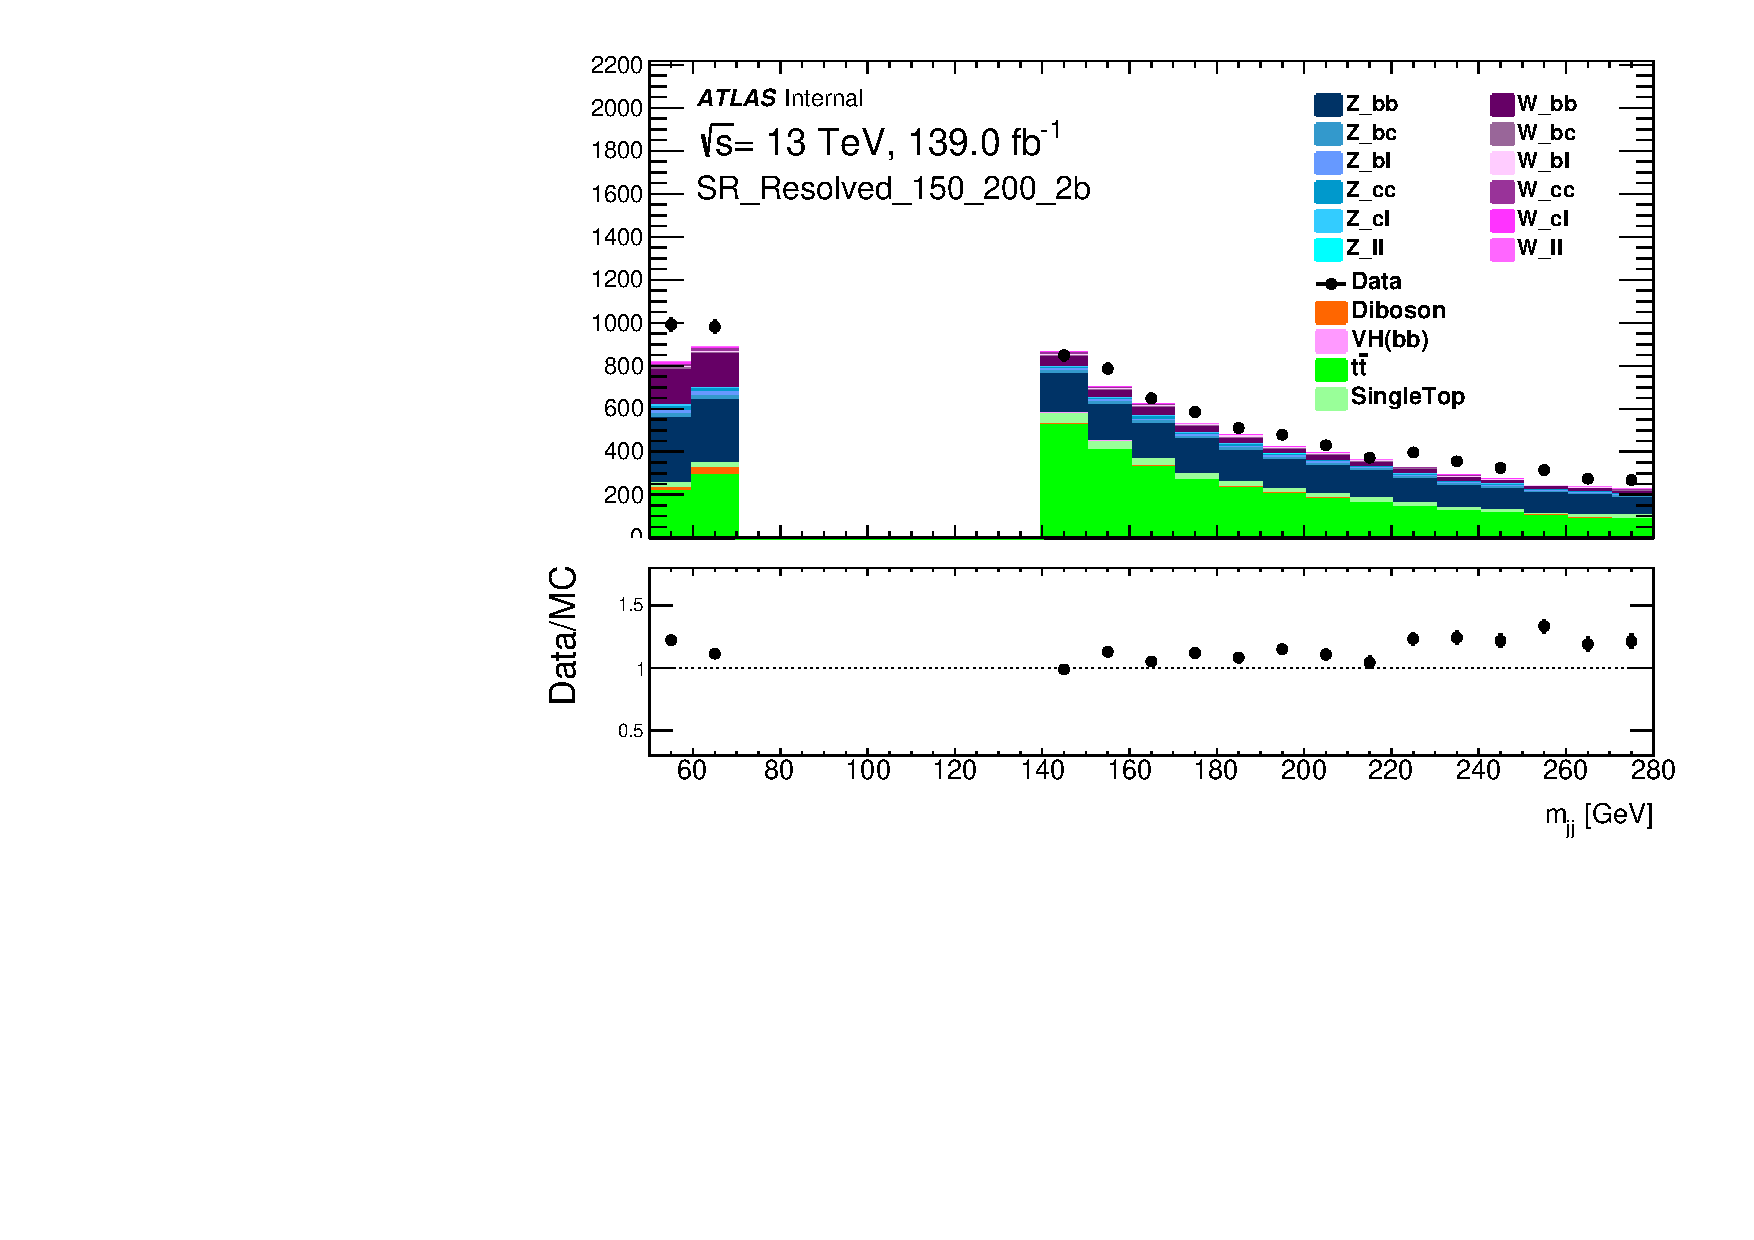
\includegraphics[width=0.46\linewidth]{chapters/c8/figures/0L/DataMC_MonoH_Nominal_SR_Resolved_150_200_2b_m_jj_10GeV.pdf}
    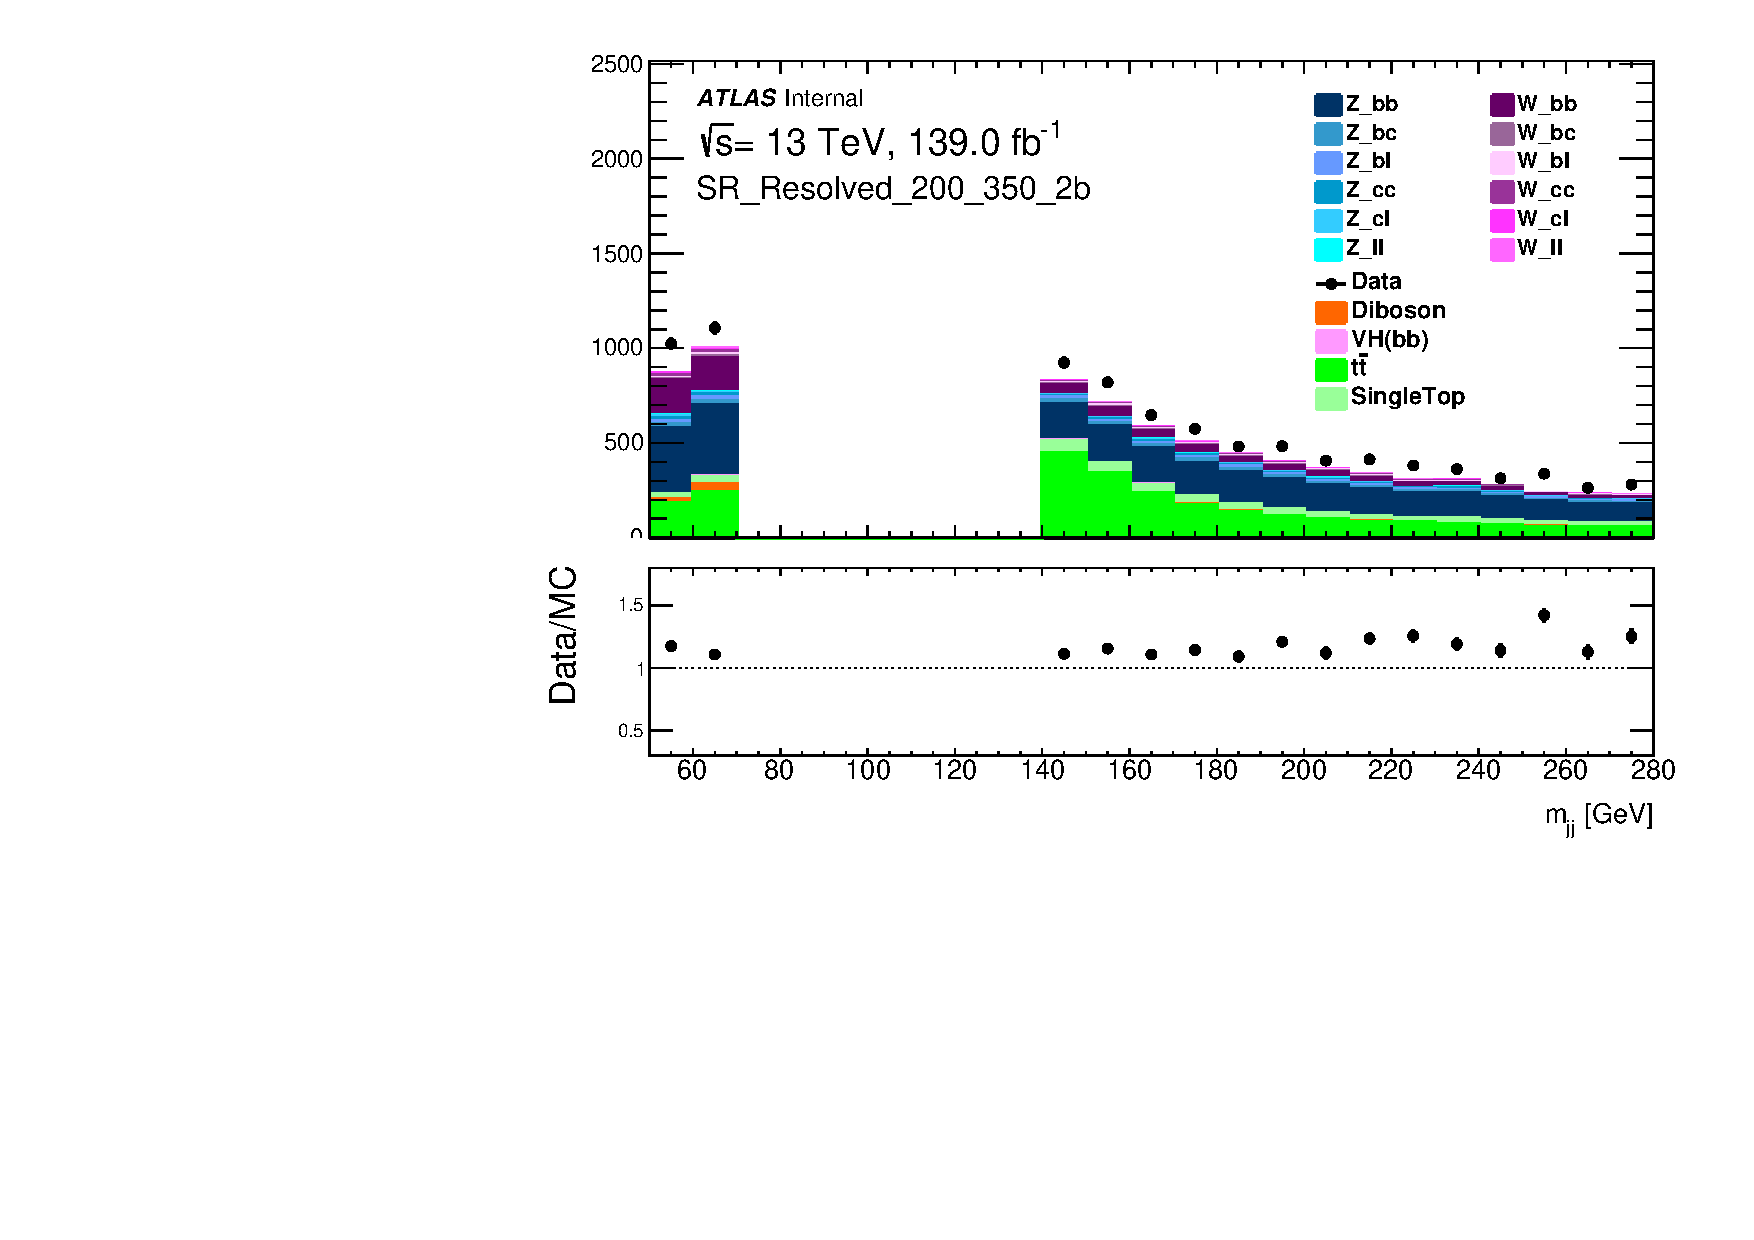
\includegraphics[width=0.46\linewidth]{chapters/c8/figures/0L/DataMC_MonoH_Nominal_SR_Resolved_200_350_2b_m_jj_10GeV.pdf}\\
    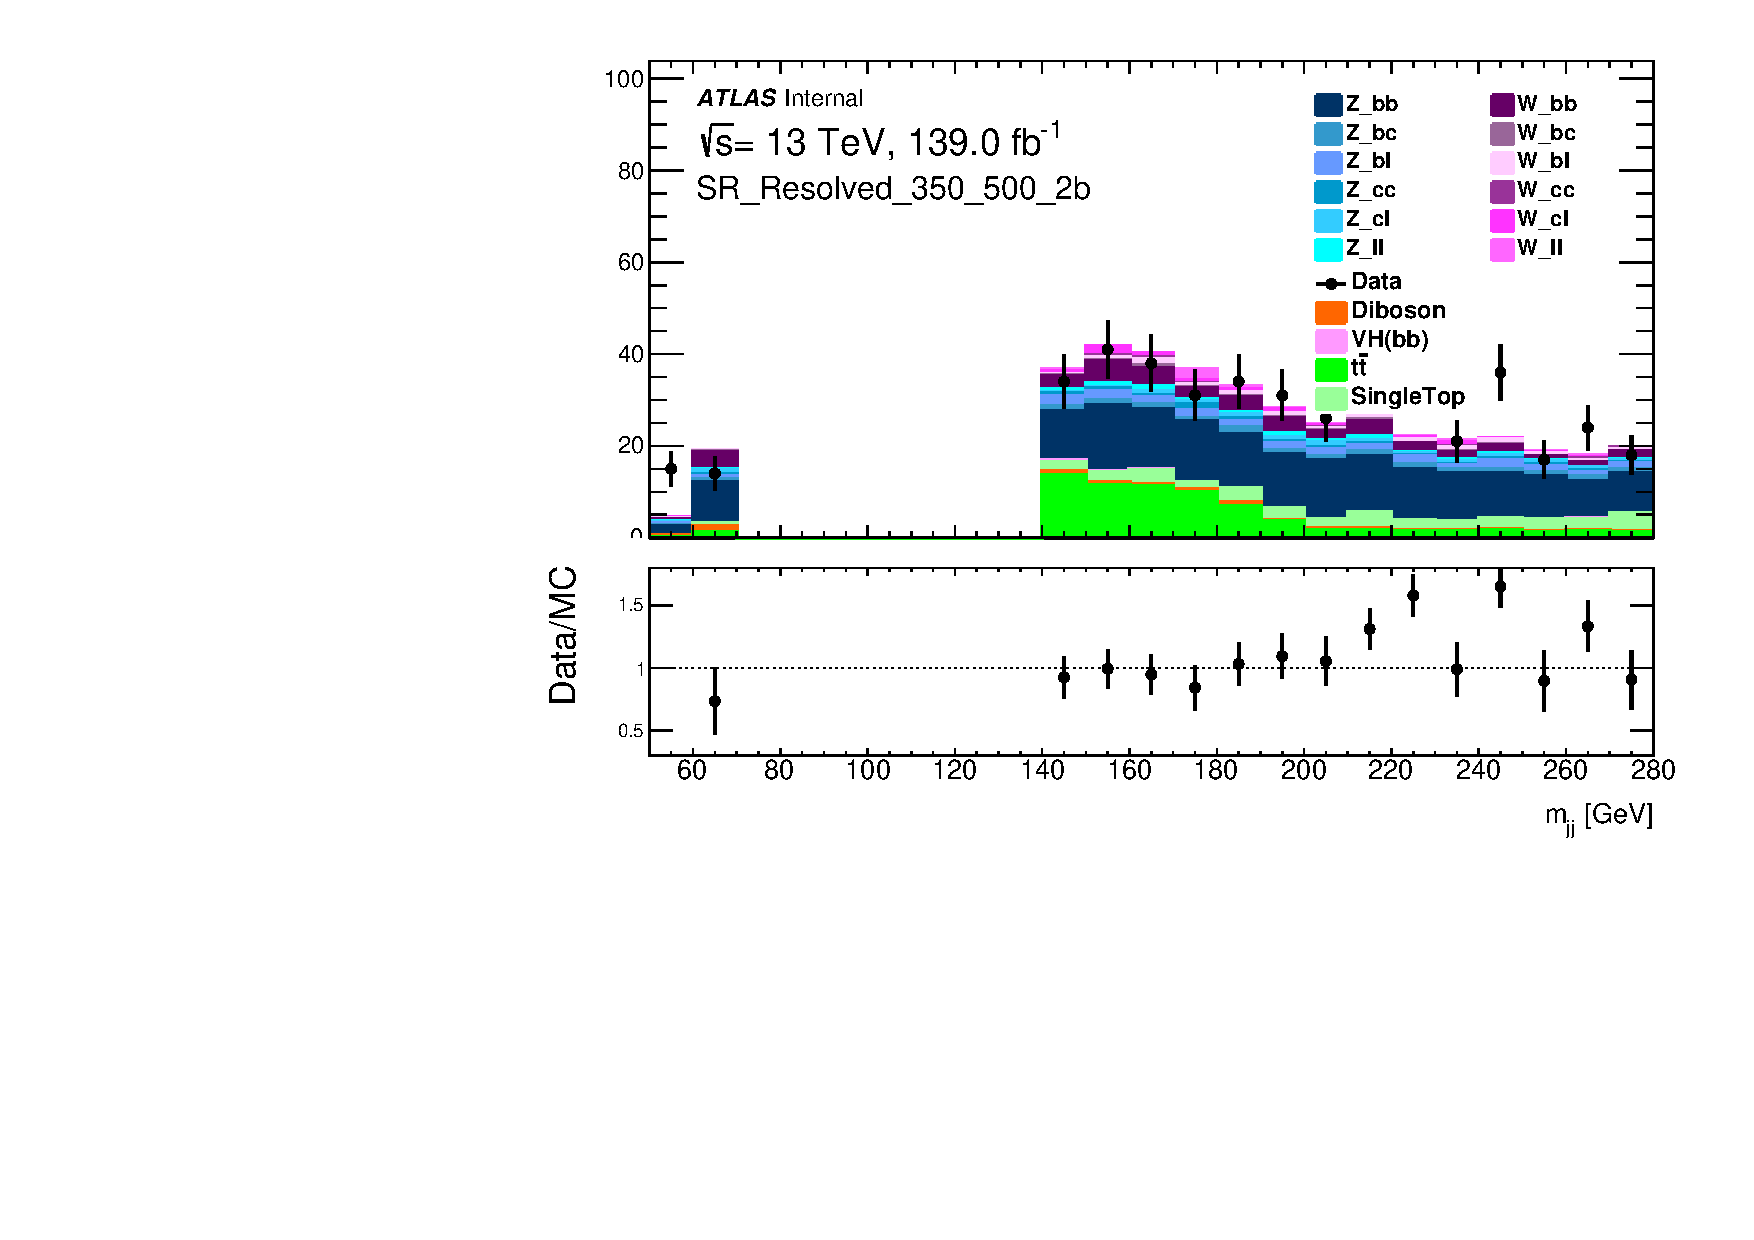
\includegraphics[width=0.46\linewidth]{chapters/c8/figures/0L/DataMC_MonoH_Nominal_SR_Resolved_350_500_2b_m_jj_10GeV.pdf}
    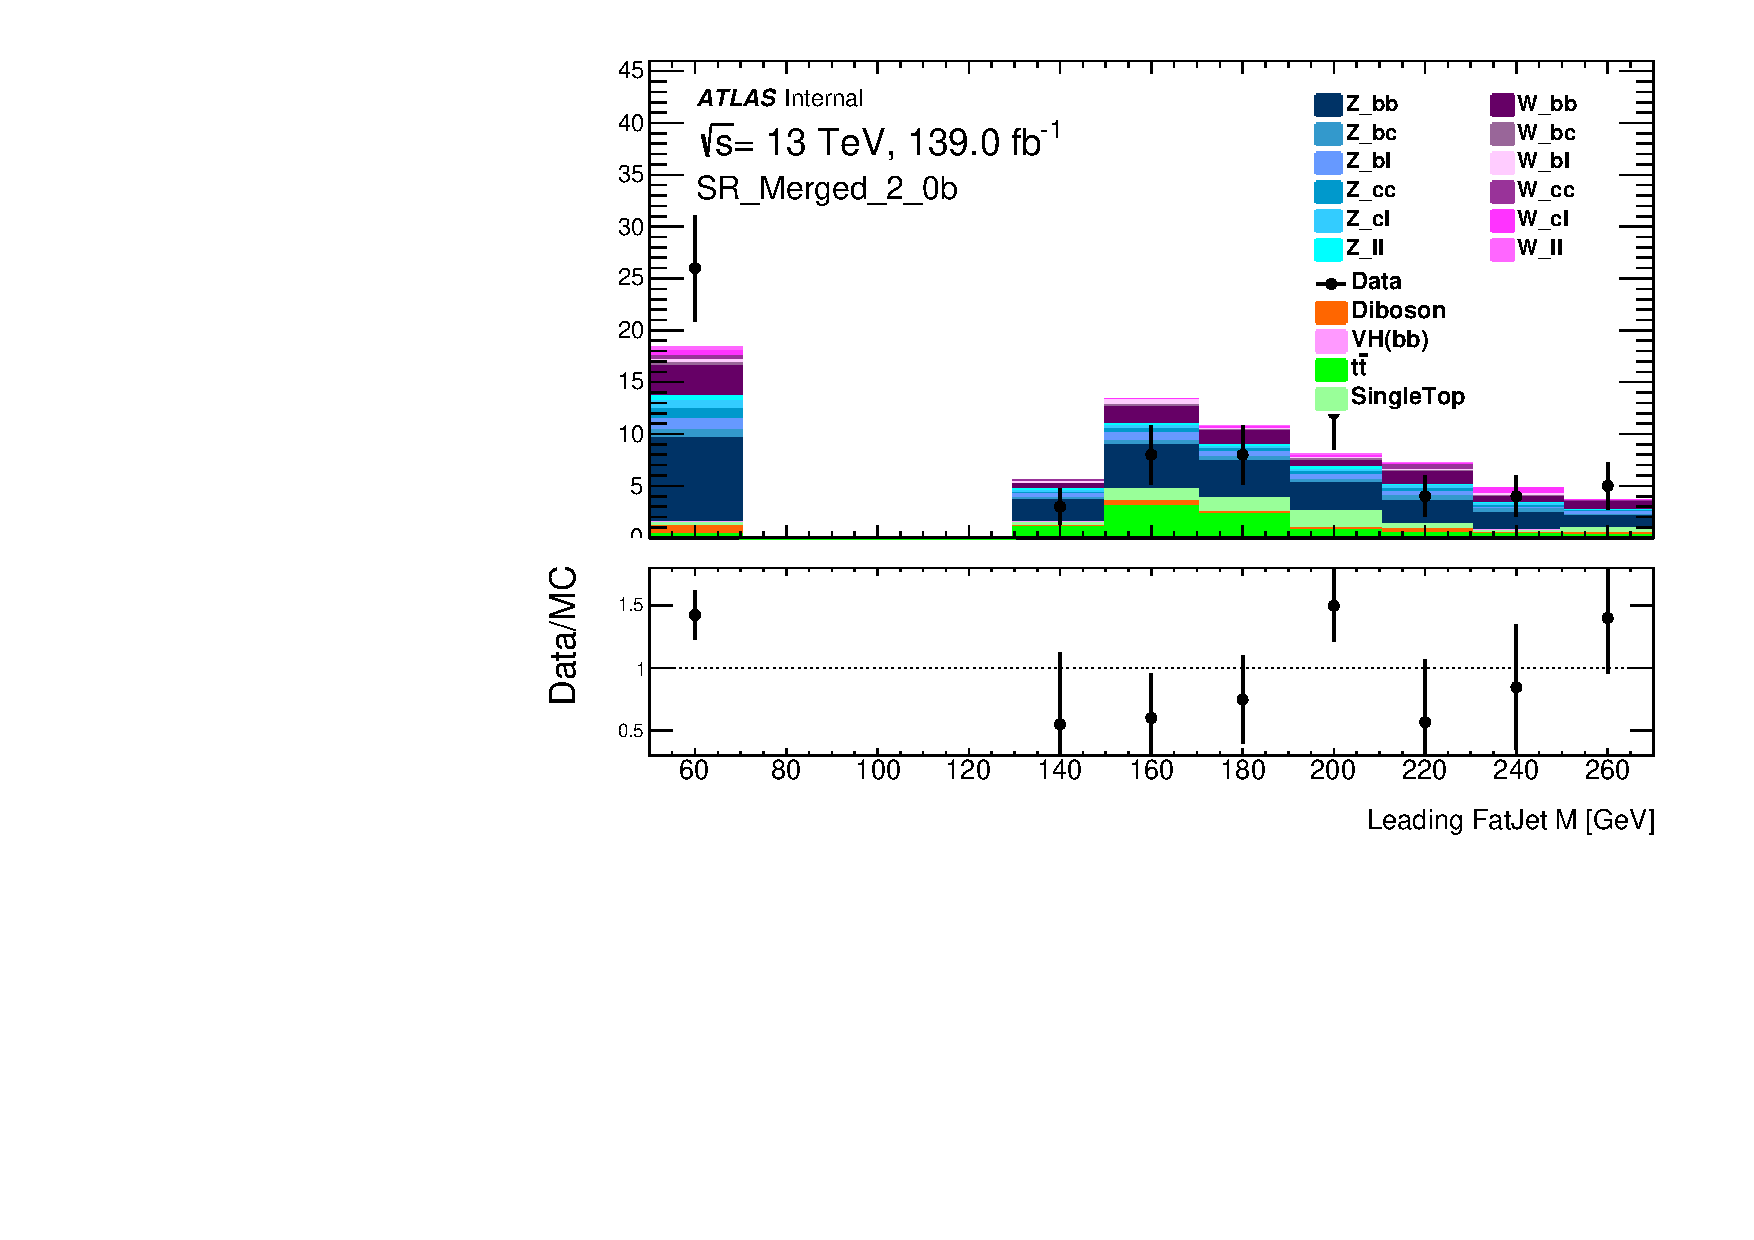
\includegraphics[width=0.46\linewidth]{chapters/c8/figures/0L/DataMC_MonoH_Nominal_SR_Merged_2_0b_fatjets_m1_20GeV.pdf}
    \caption{Higgs candidate mass spectra in the different \met regions with 2 $b$-tagged jets in the 0-lepton channel.}
    \label{fig:data-mc-0l-mjj-2b}
\end{figure}

\begin{figure}[!htb]
    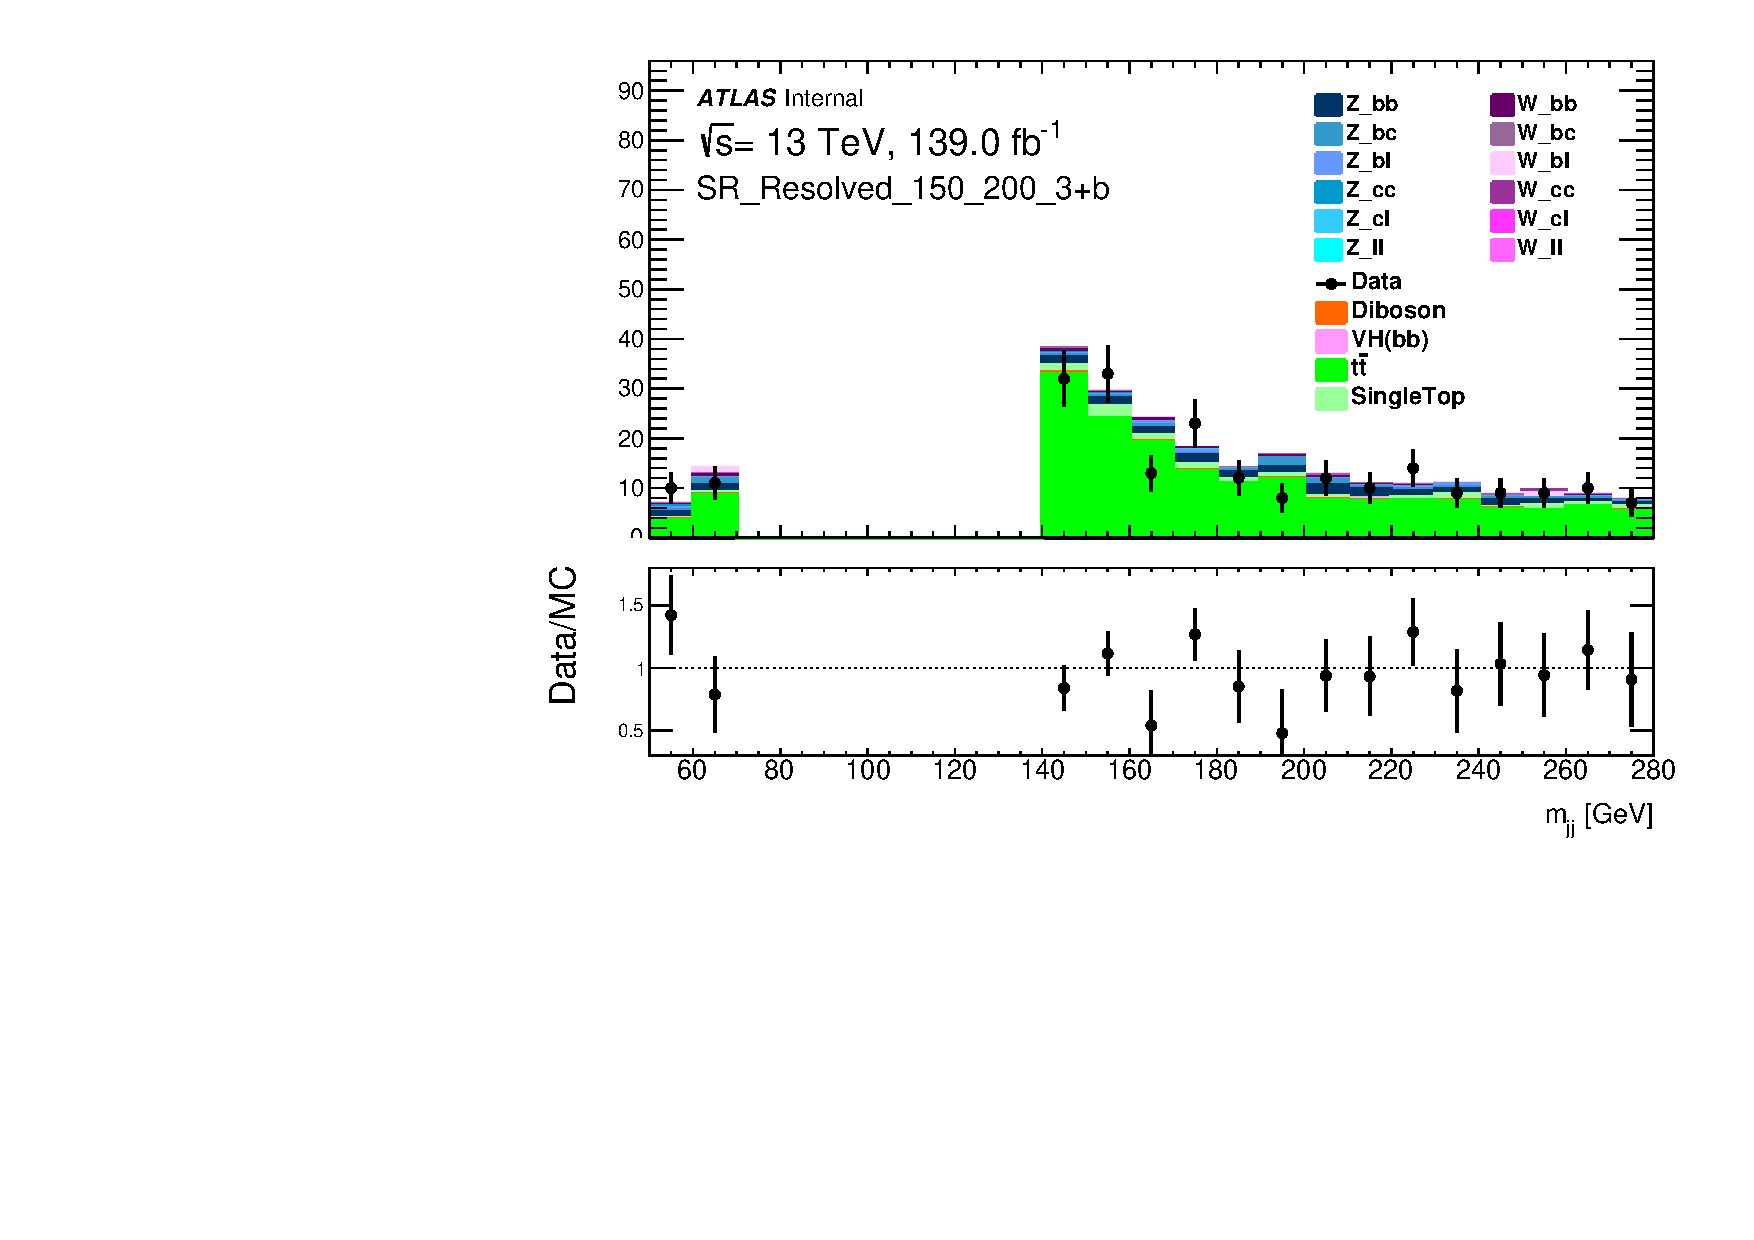
\includegraphics[width=0.46\linewidth]{chapters/c8/figures/0L/DataMC_MonoH_Nominal_SR_Resolved_150_200_3+b_m_jj_10GeV.pdf}
    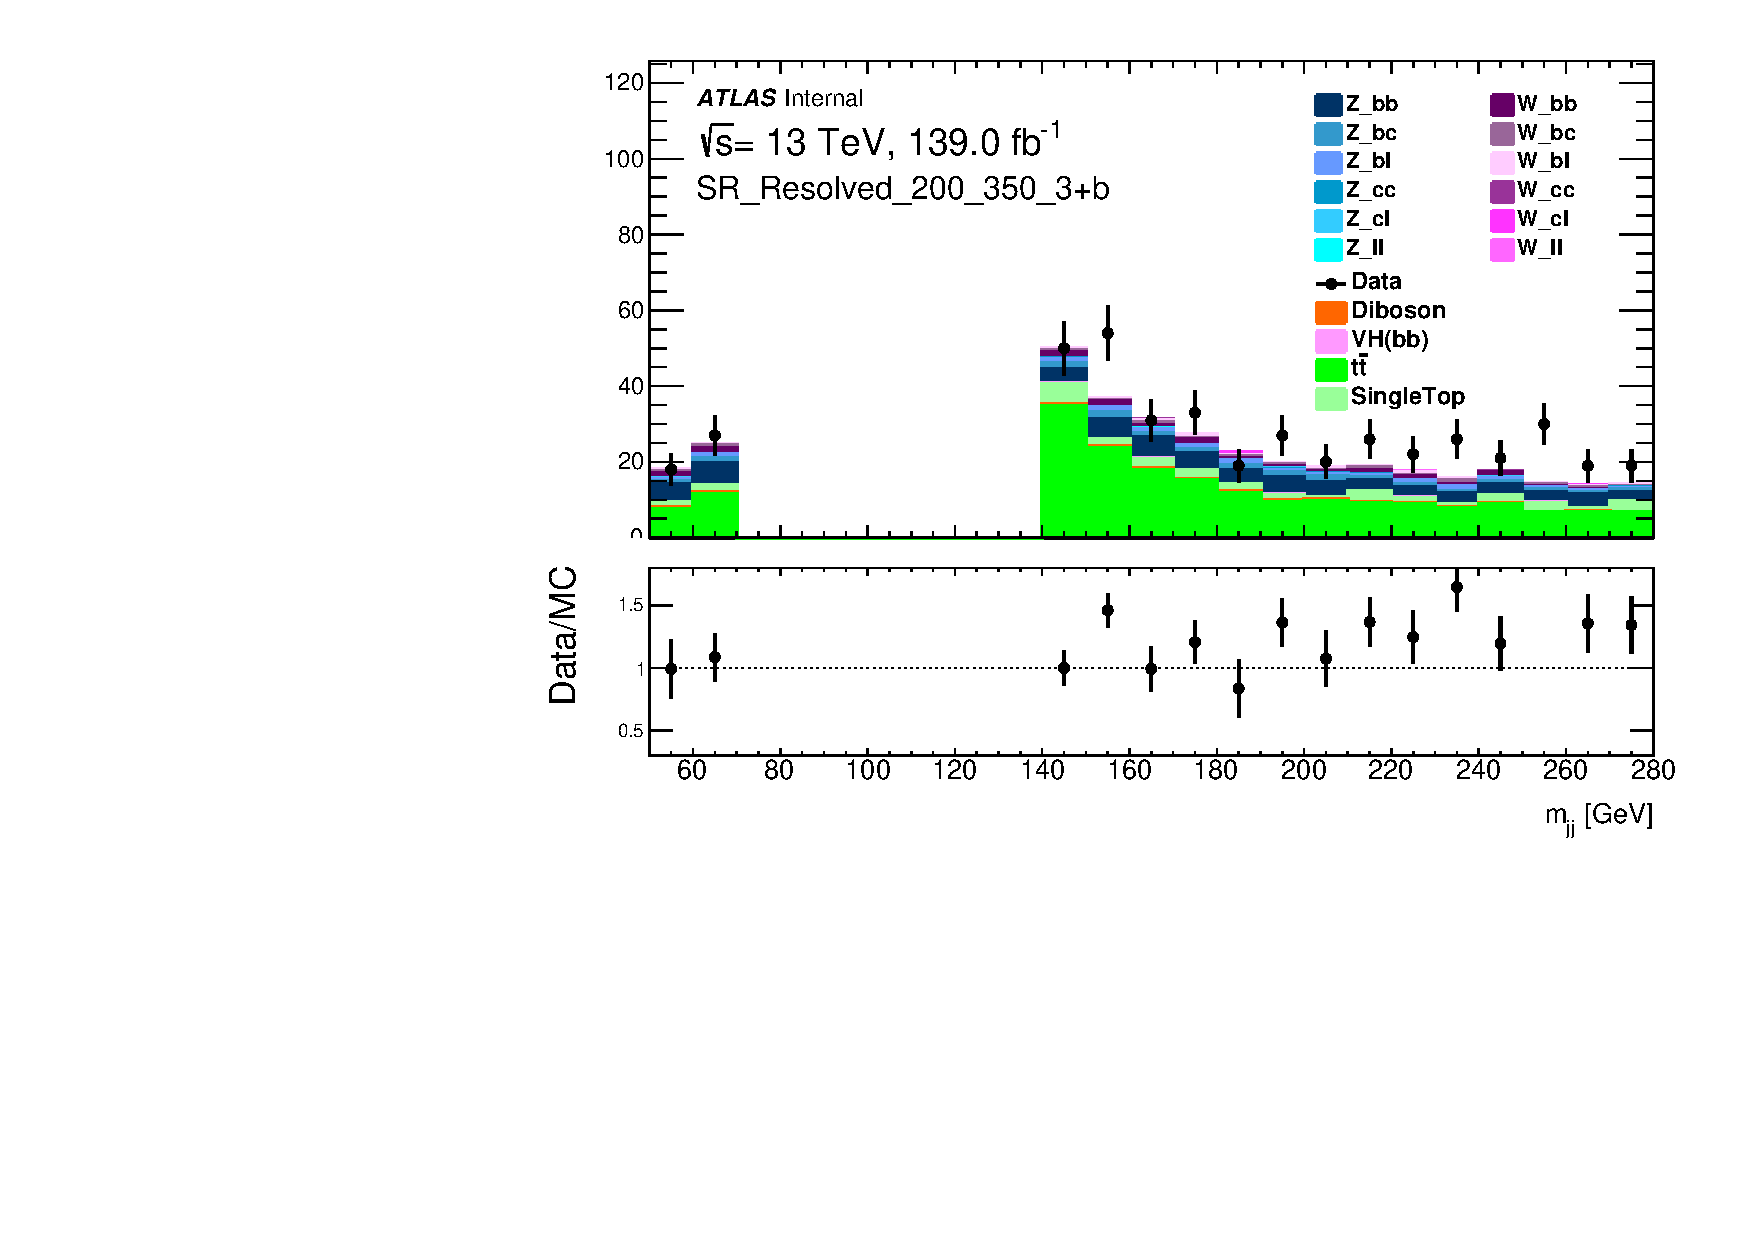
\includegraphics[width=0.46\linewidth]{chapters/c8/figures/0L/DataMC_MonoH_Nominal_SR_Resolved_200_350_3+b_m_jj_10GeV.pdf}\\
    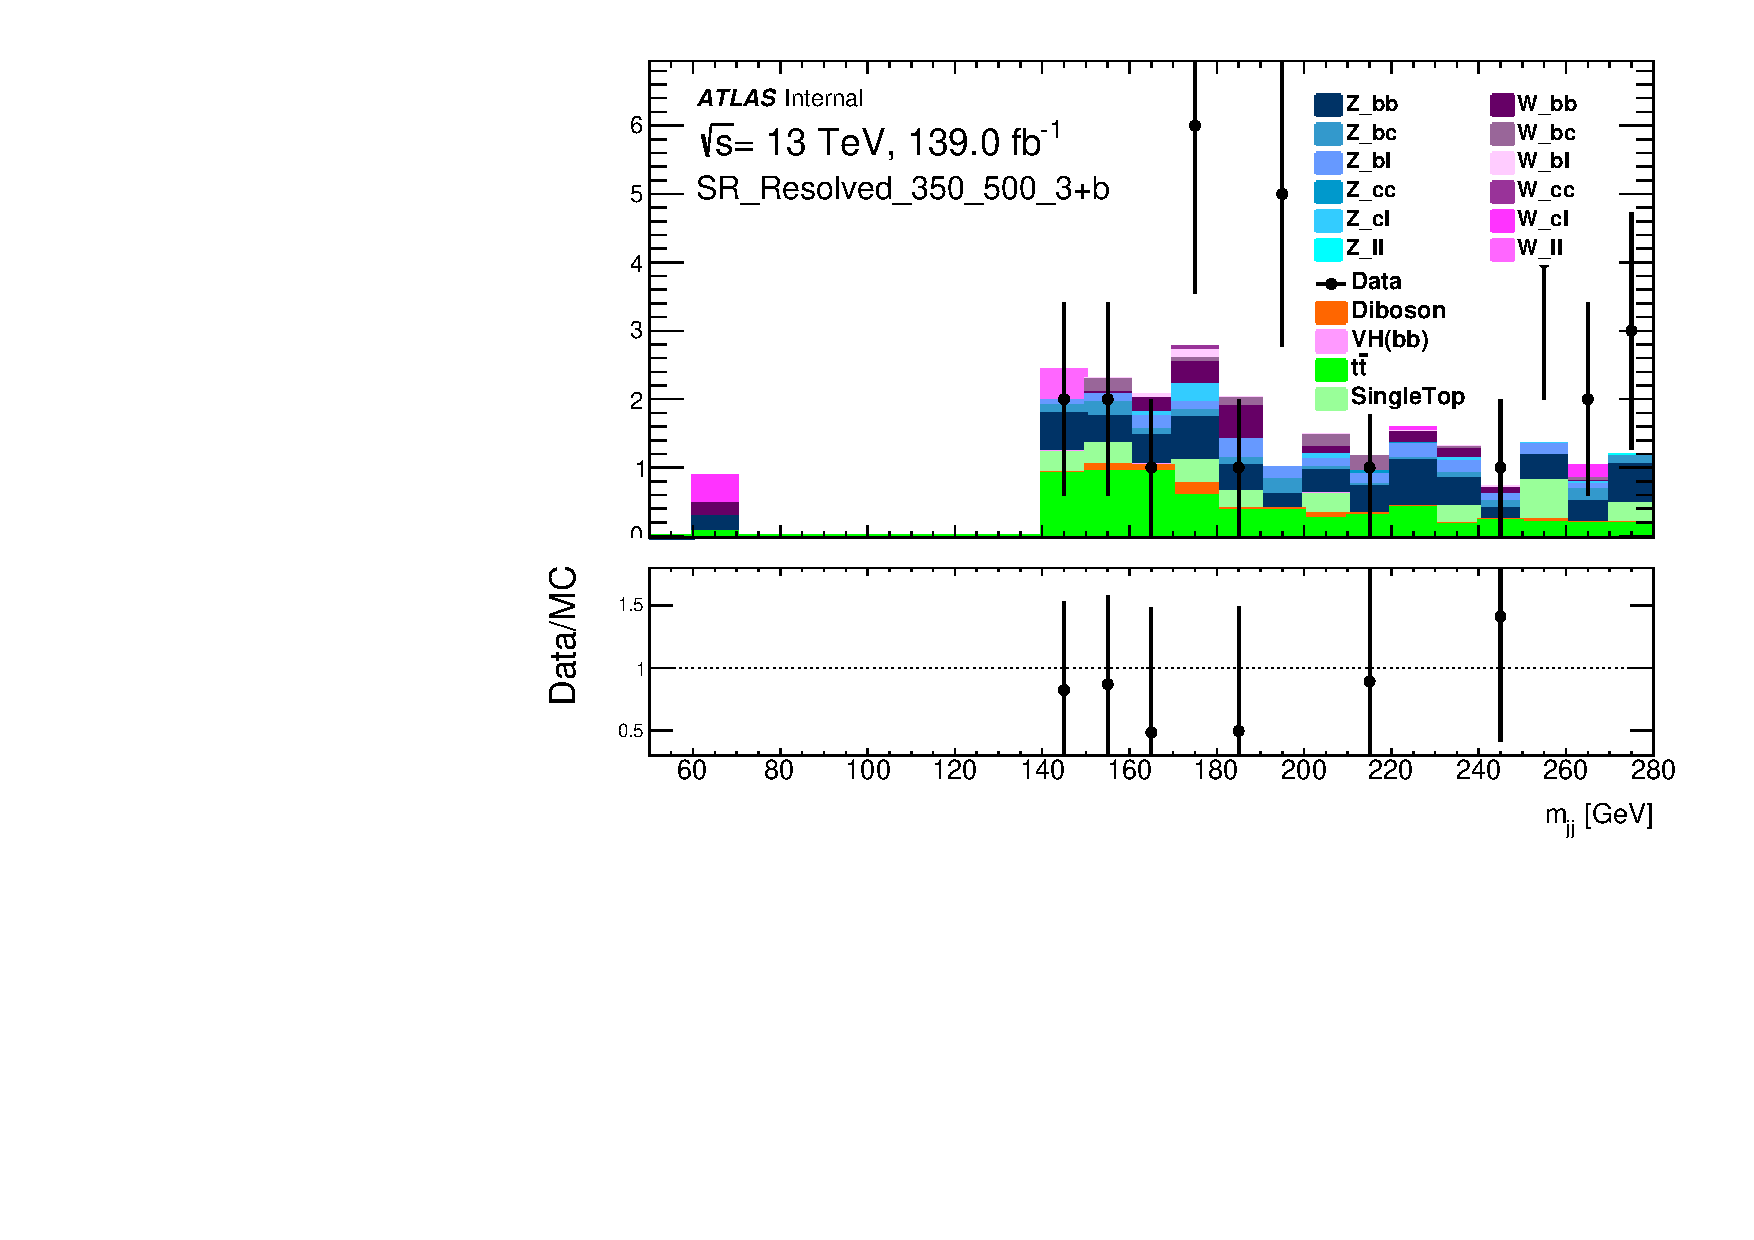
\includegraphics[width=0.46\linewidth]{chapters/c8/figures/0L/DataMC_MonoH_Nominal_SR_Resolved_350_500_3+b_m_jj_10GeV.pdf}
    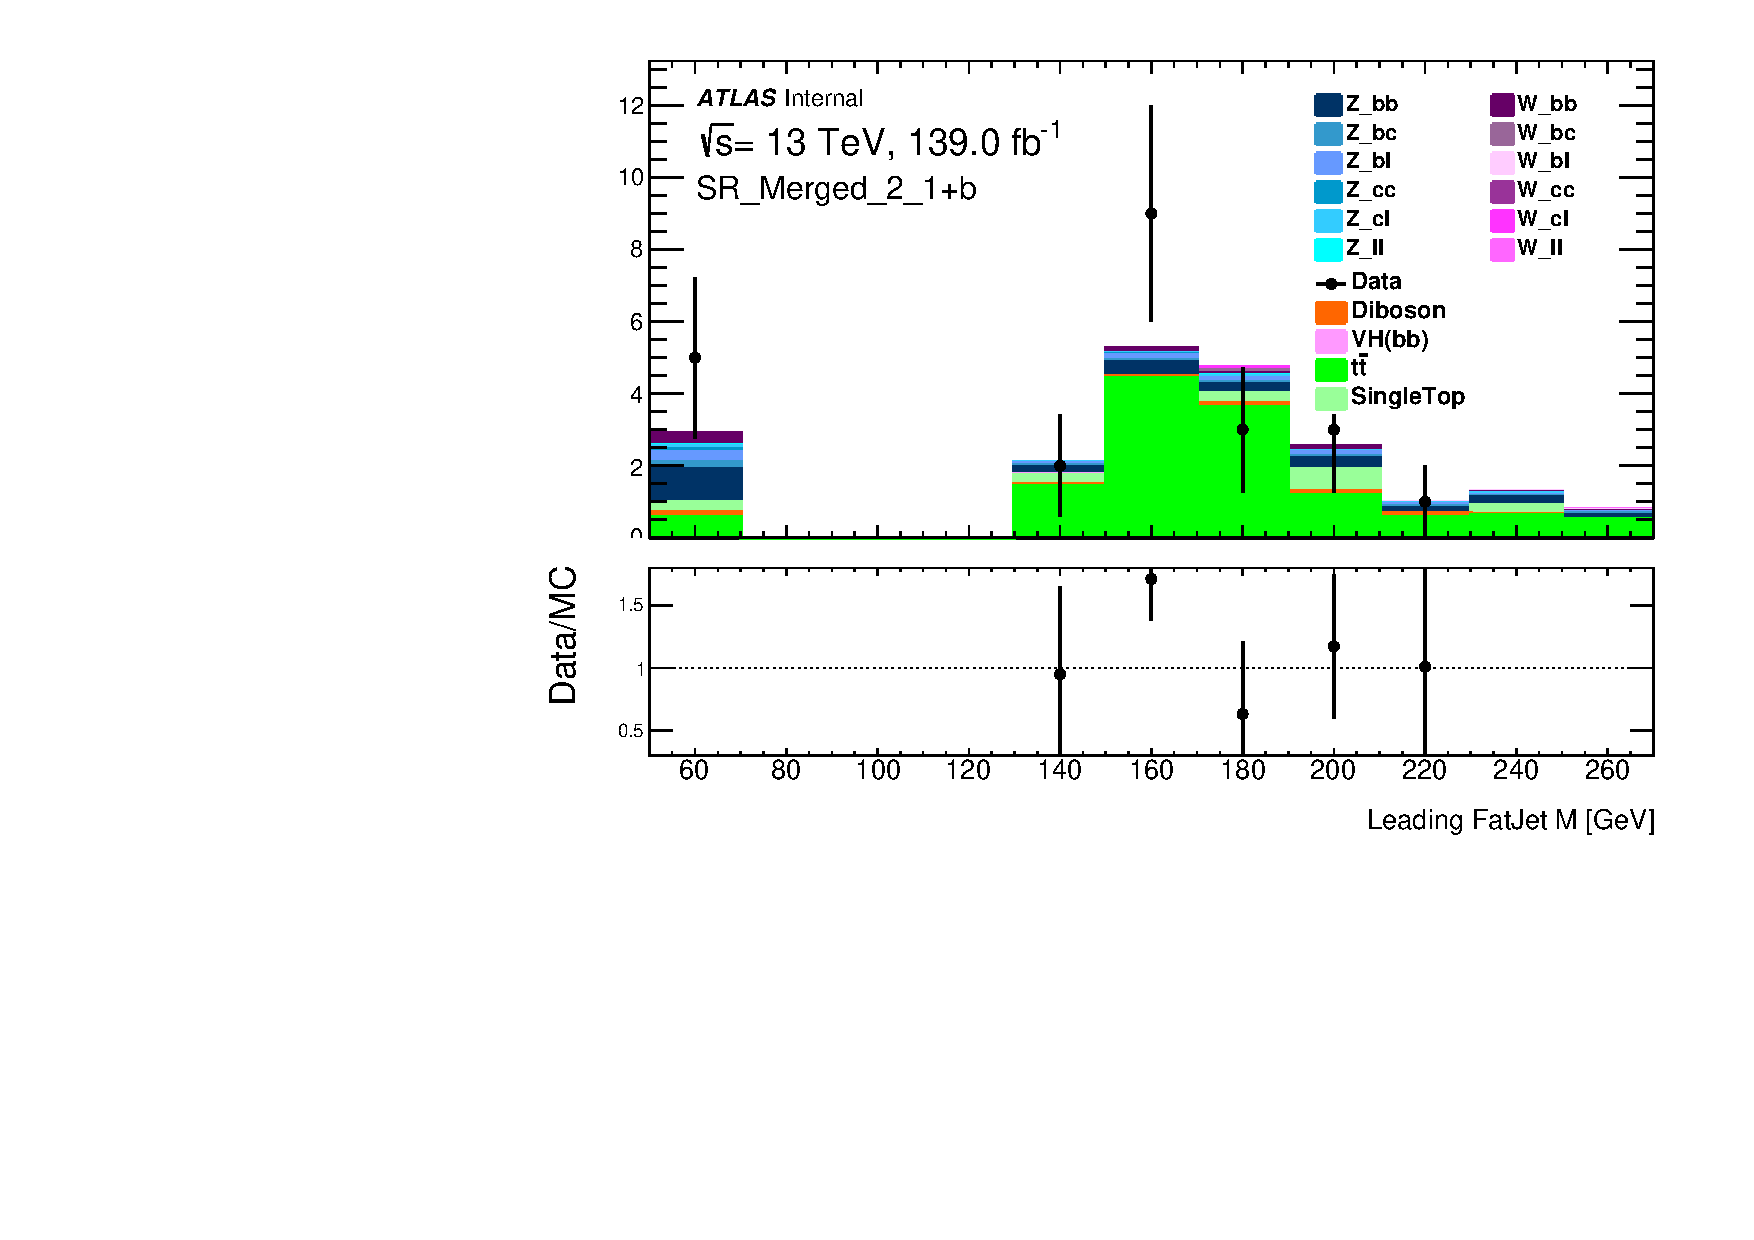
\includegraphics[width=0.46\linewidth]{chapters/c8/figures/0L/DataMC_MonoH_Nominal_SR_Merged_2_1+b_fatjets_m1_20GeV.pdf}
    \caption{Higgs candidate mass spectra in the different \met regions with at least 3 $b$-tagged jets in the 0-lepton channel.}
    \label{fig:data-mc-0l-mjj-3+b}
\end{figure}

\subsection{Control region: 1-lepton}

\begin{figure}[!htb]
    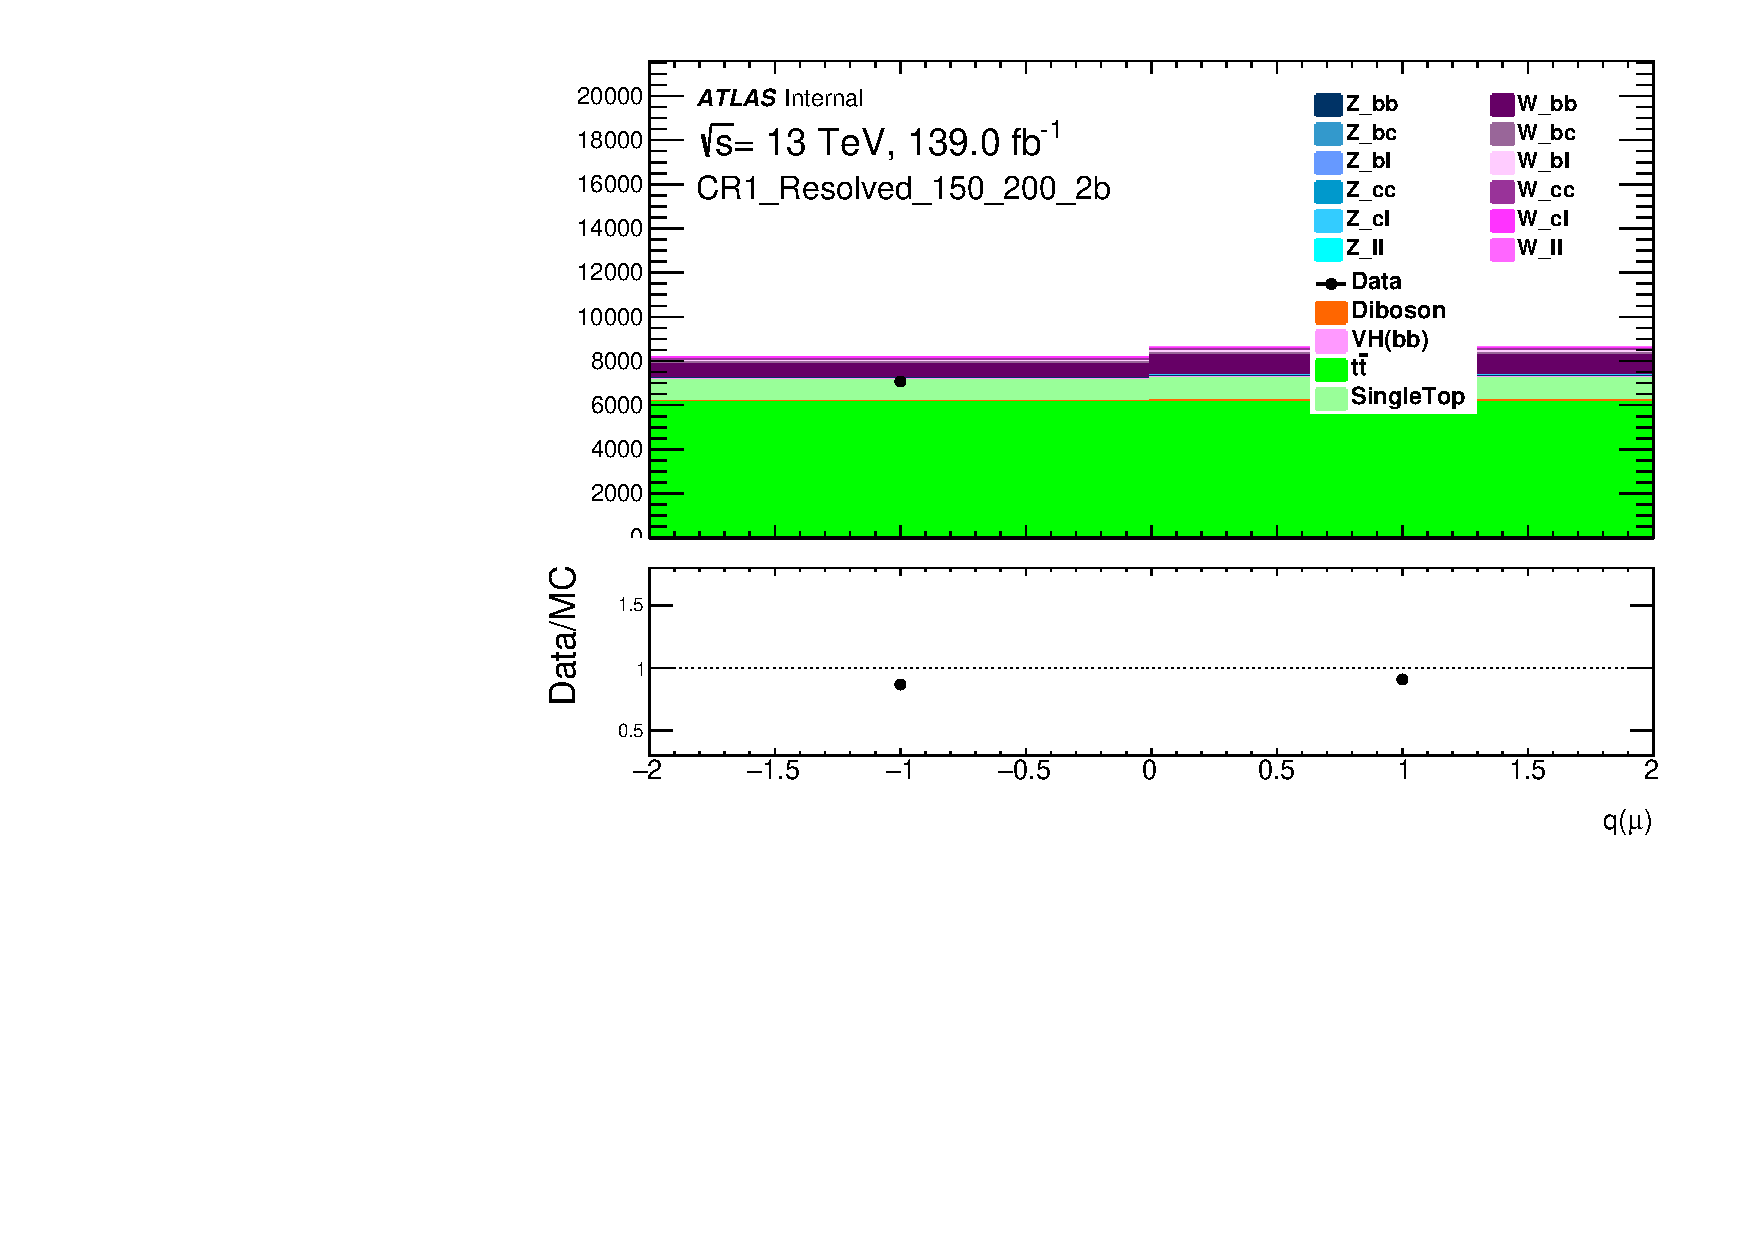
\includegraphics[width=0.46\linewidth]{chapters/c8/figures/1L/DataMC_MonoH_Nominal_CR1_Resolved_150_200_2b_mu_charge.pdf}
    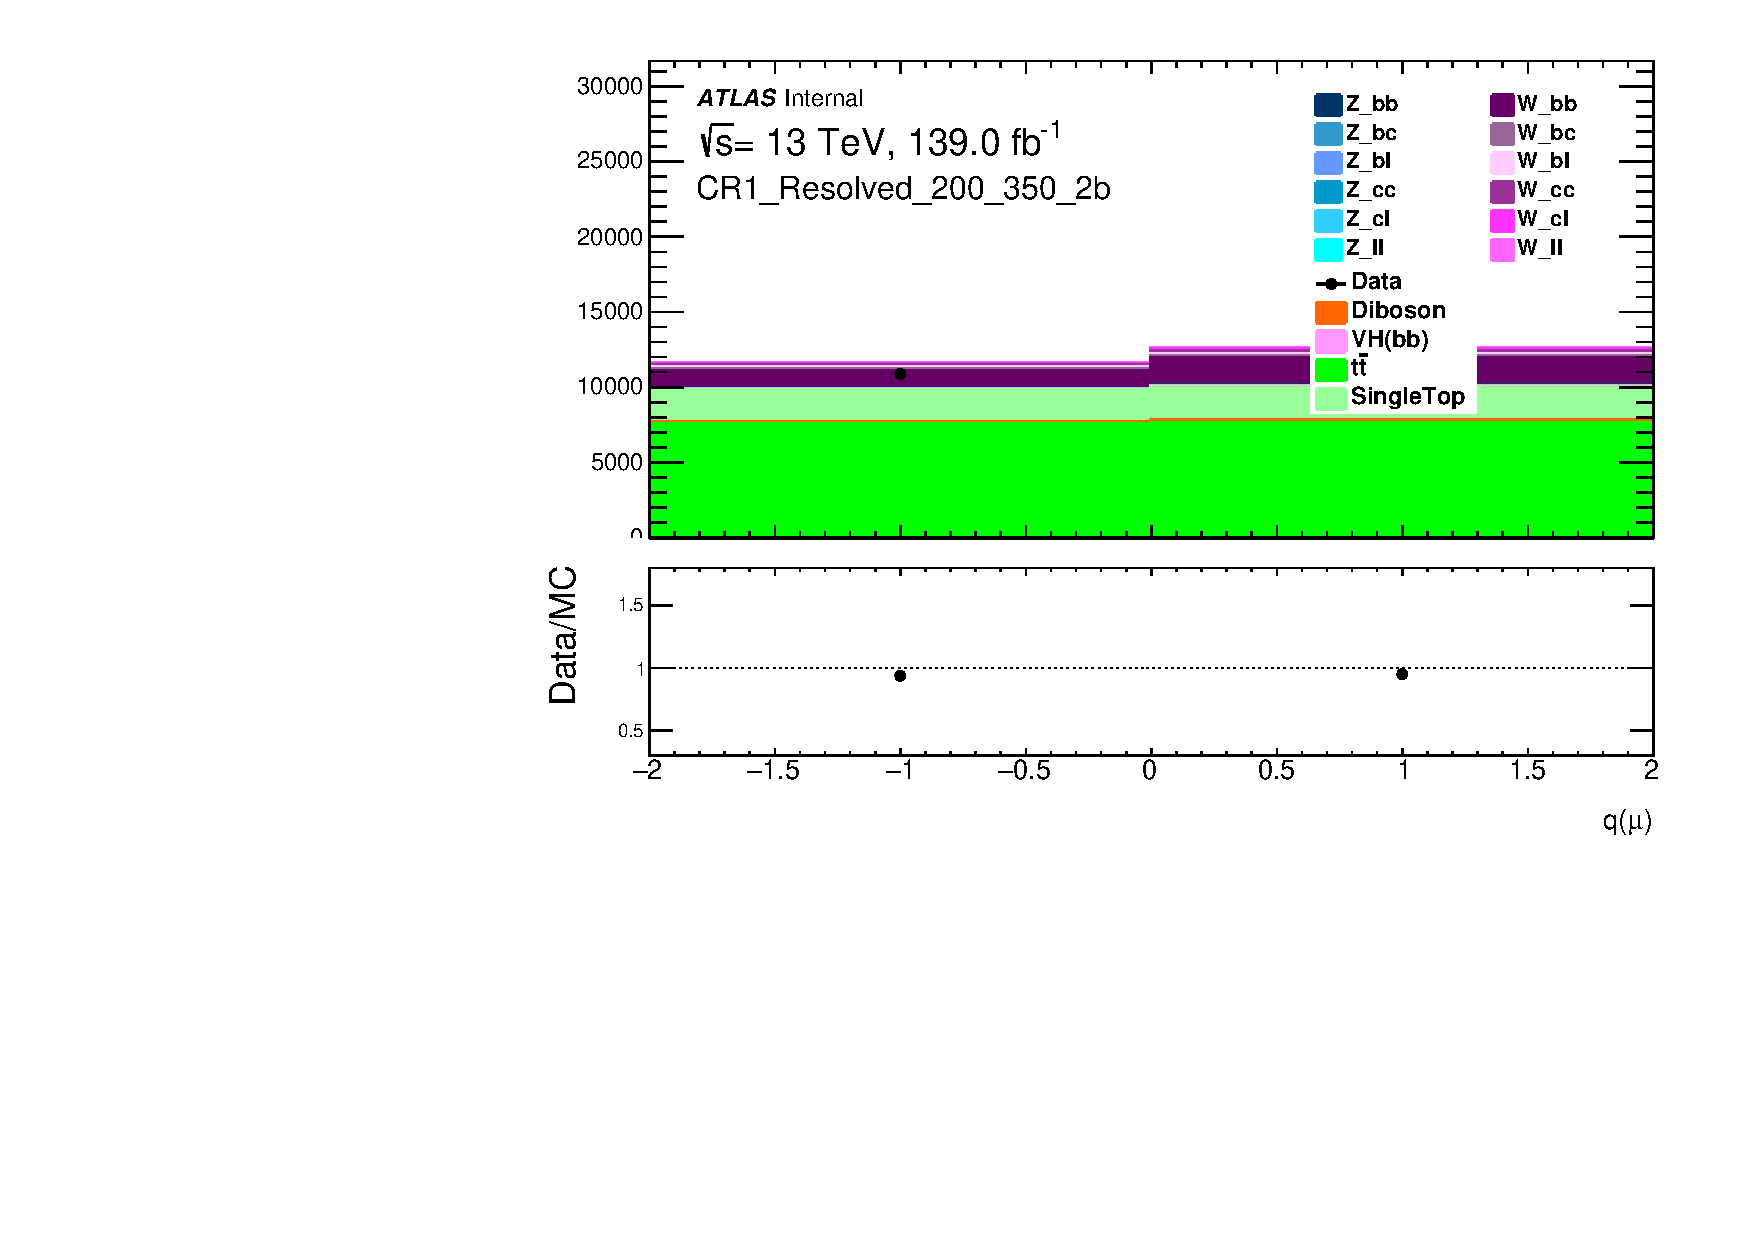
\includegraphics[width=0.46\linewidth]{chapters/c8/figures/1L/DataMC_MonoH_Nominal_CR1_Resolved_200_350_2b_mu_charge.pdf}\\
    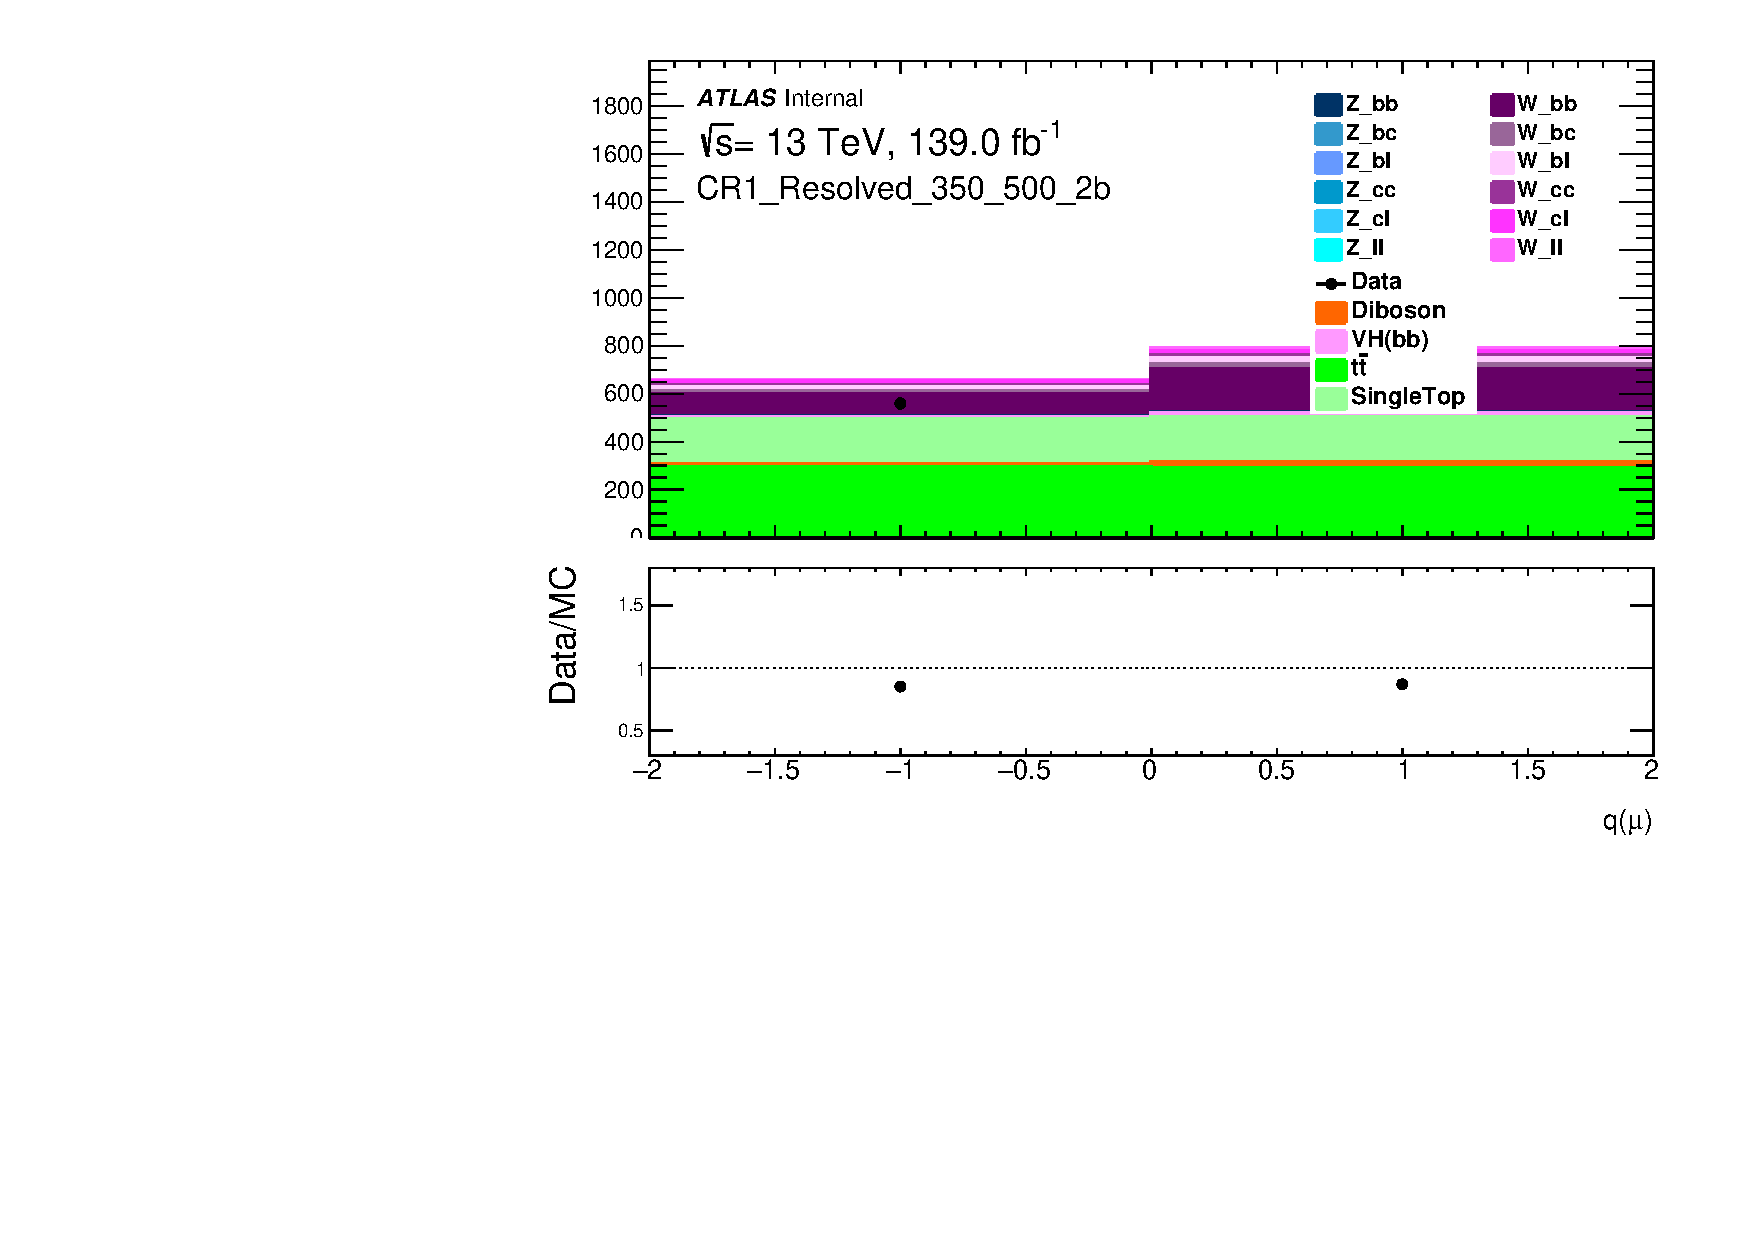
\includegraphics[width=0.46\linewidth]{chapters/c8/figures/1L/DataMC_MonoH_Nominal_CR1_Resolved_350_500_2b_mu_charge.pdf}
    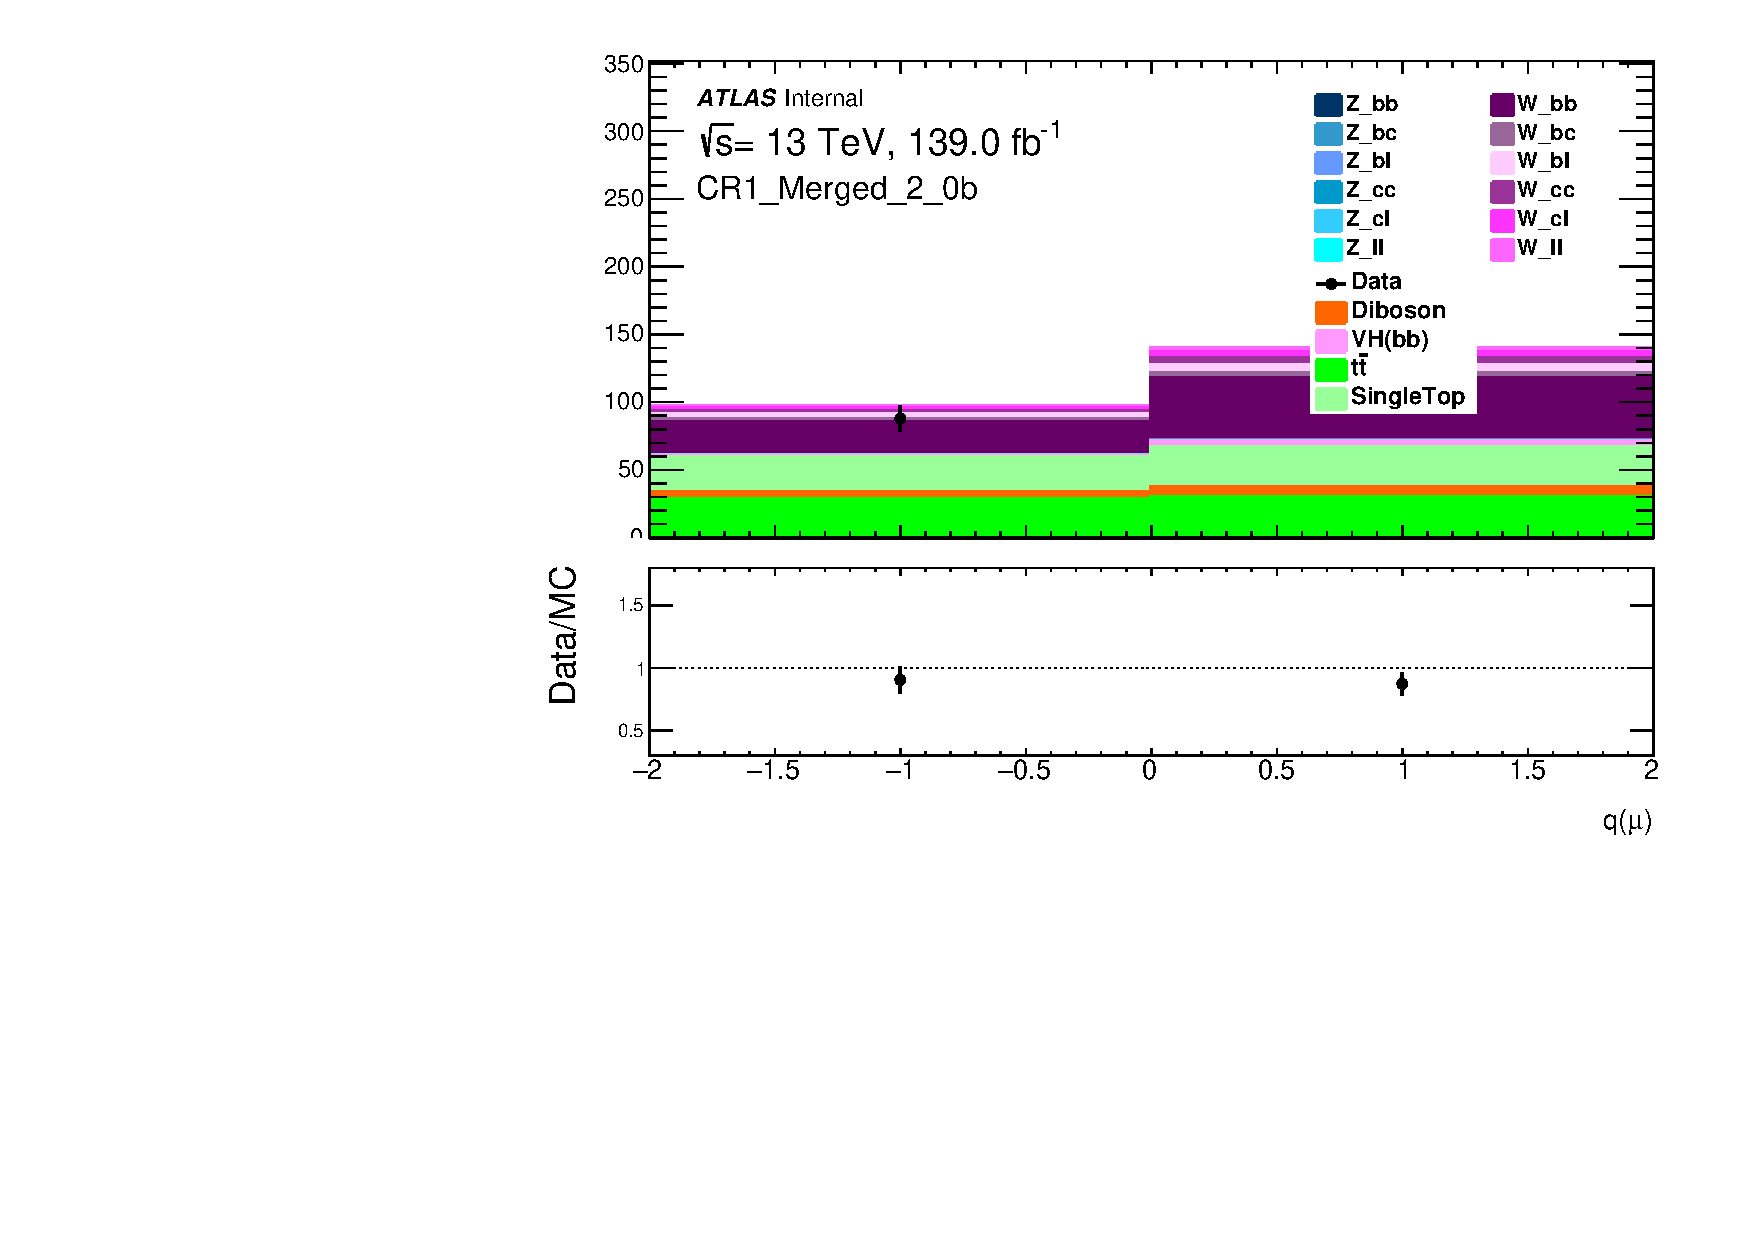
\includegraphics[width=0.46\linewidth]{chapters/c8/figures/1L/DataMC_MonoH_Nominal_CR1_Merged_2_0b_mu_charge.pdf}
    \caption{Muon charge distribution in the different \met regions with 2 $b$-tagged jets in the 1-lepton channel.}
    \label{fig:data-mc-1l-mu-charge-2b}
\end{figure}

\begin{figure}[!htb]
    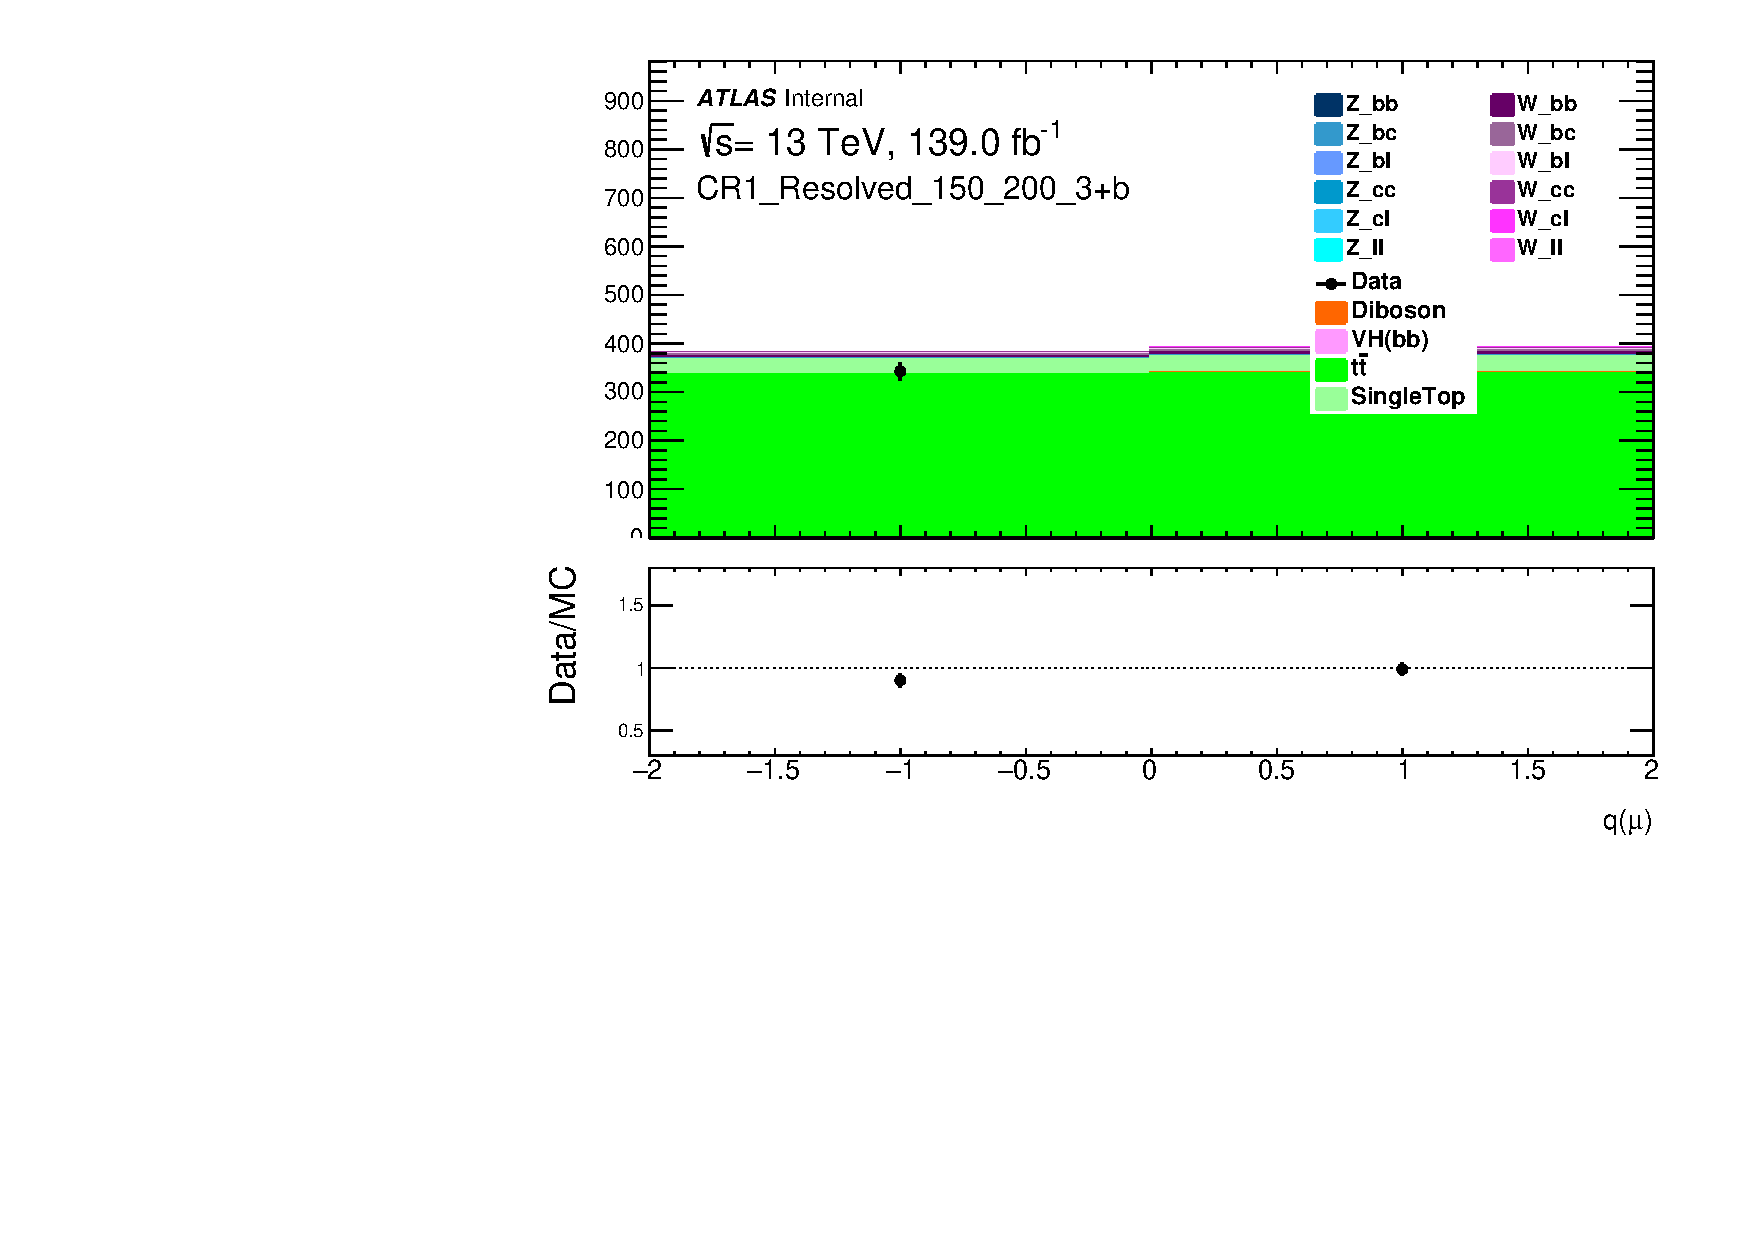
\includegraphics[width=0.46\linewidth]{chapters/c8/figures/1L/DataMC_MonoH_Nominal_CR1_Resolved_150_200_3+b_mu_charge.pdf}
    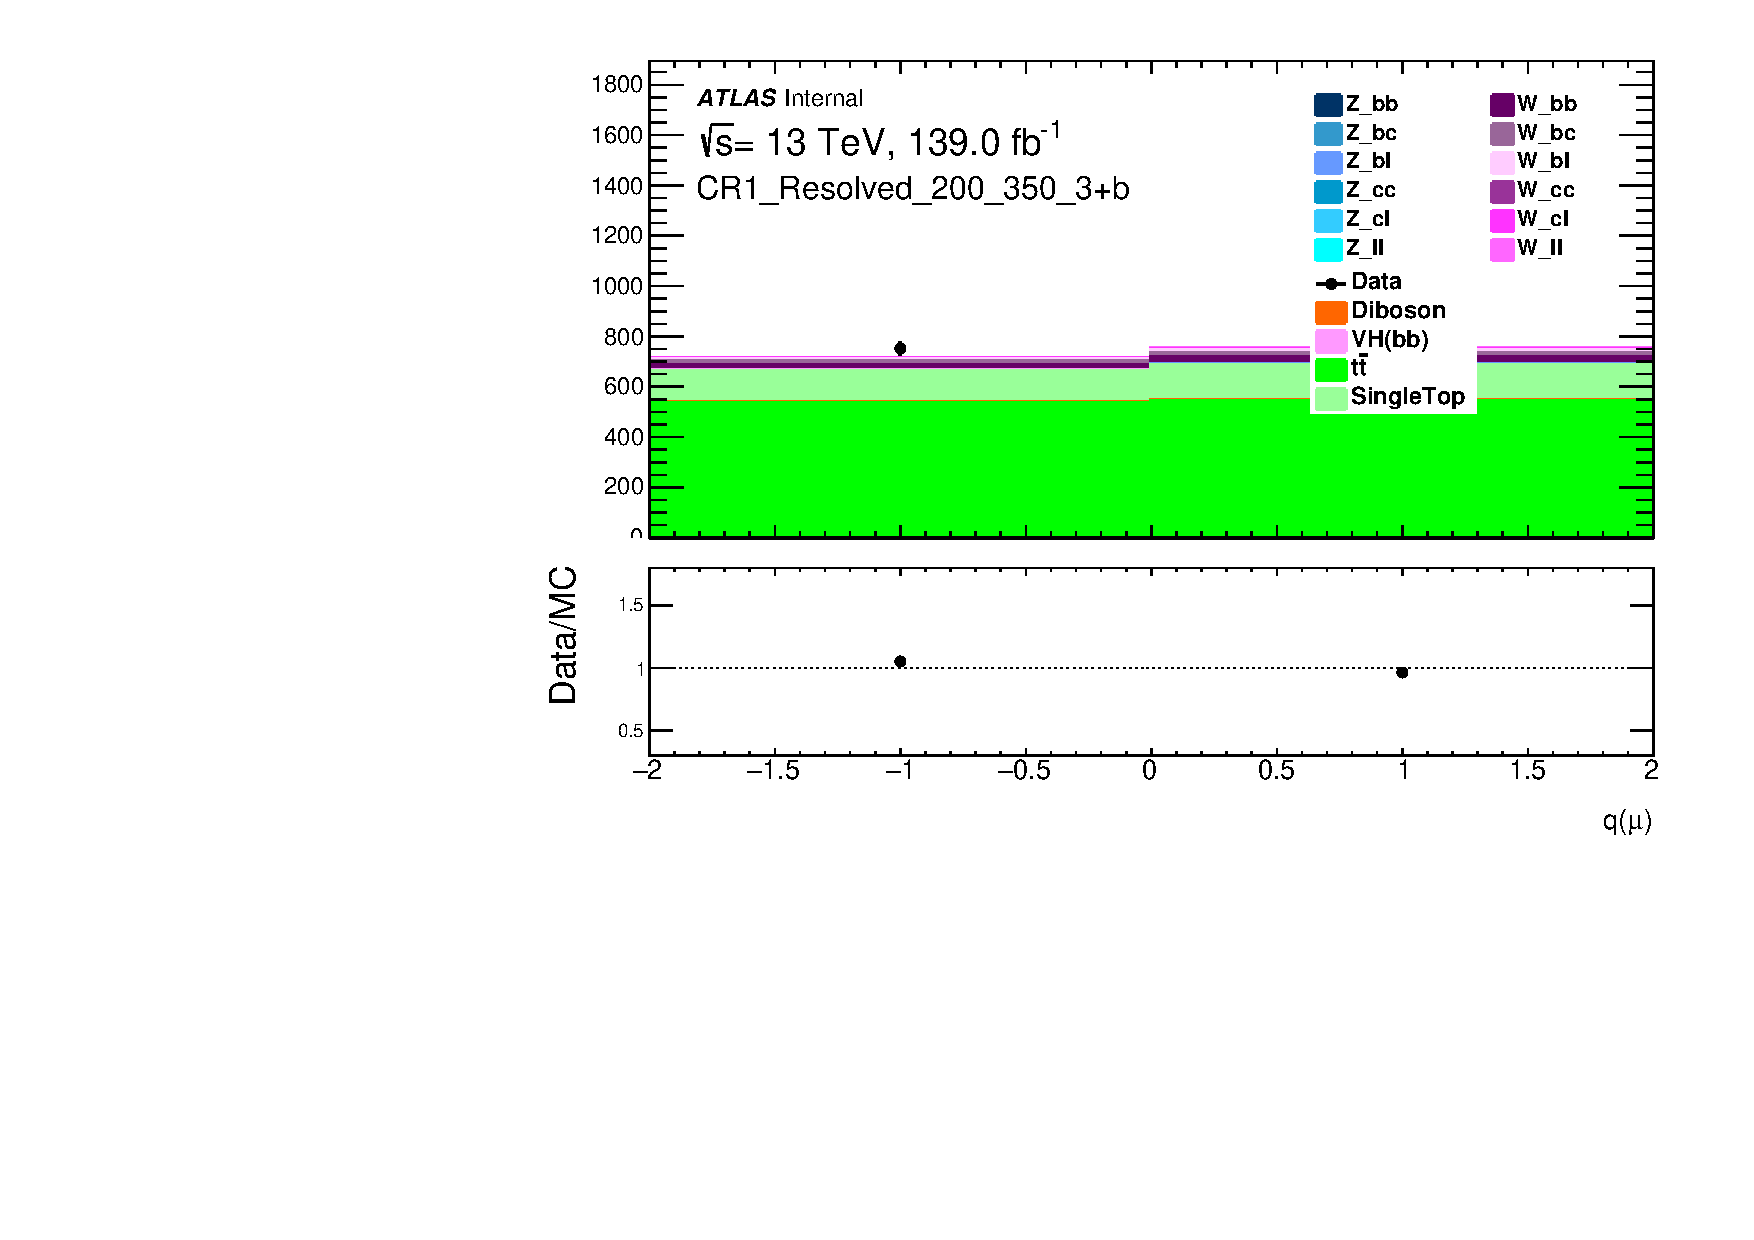
\includegraphics[width=0.46\linewidth]{chapters/c8/figures/1L/DataMC_MonoH_Nominal_CR1_Resolved_200_350_3+b_mu_charge.pdf}\\
    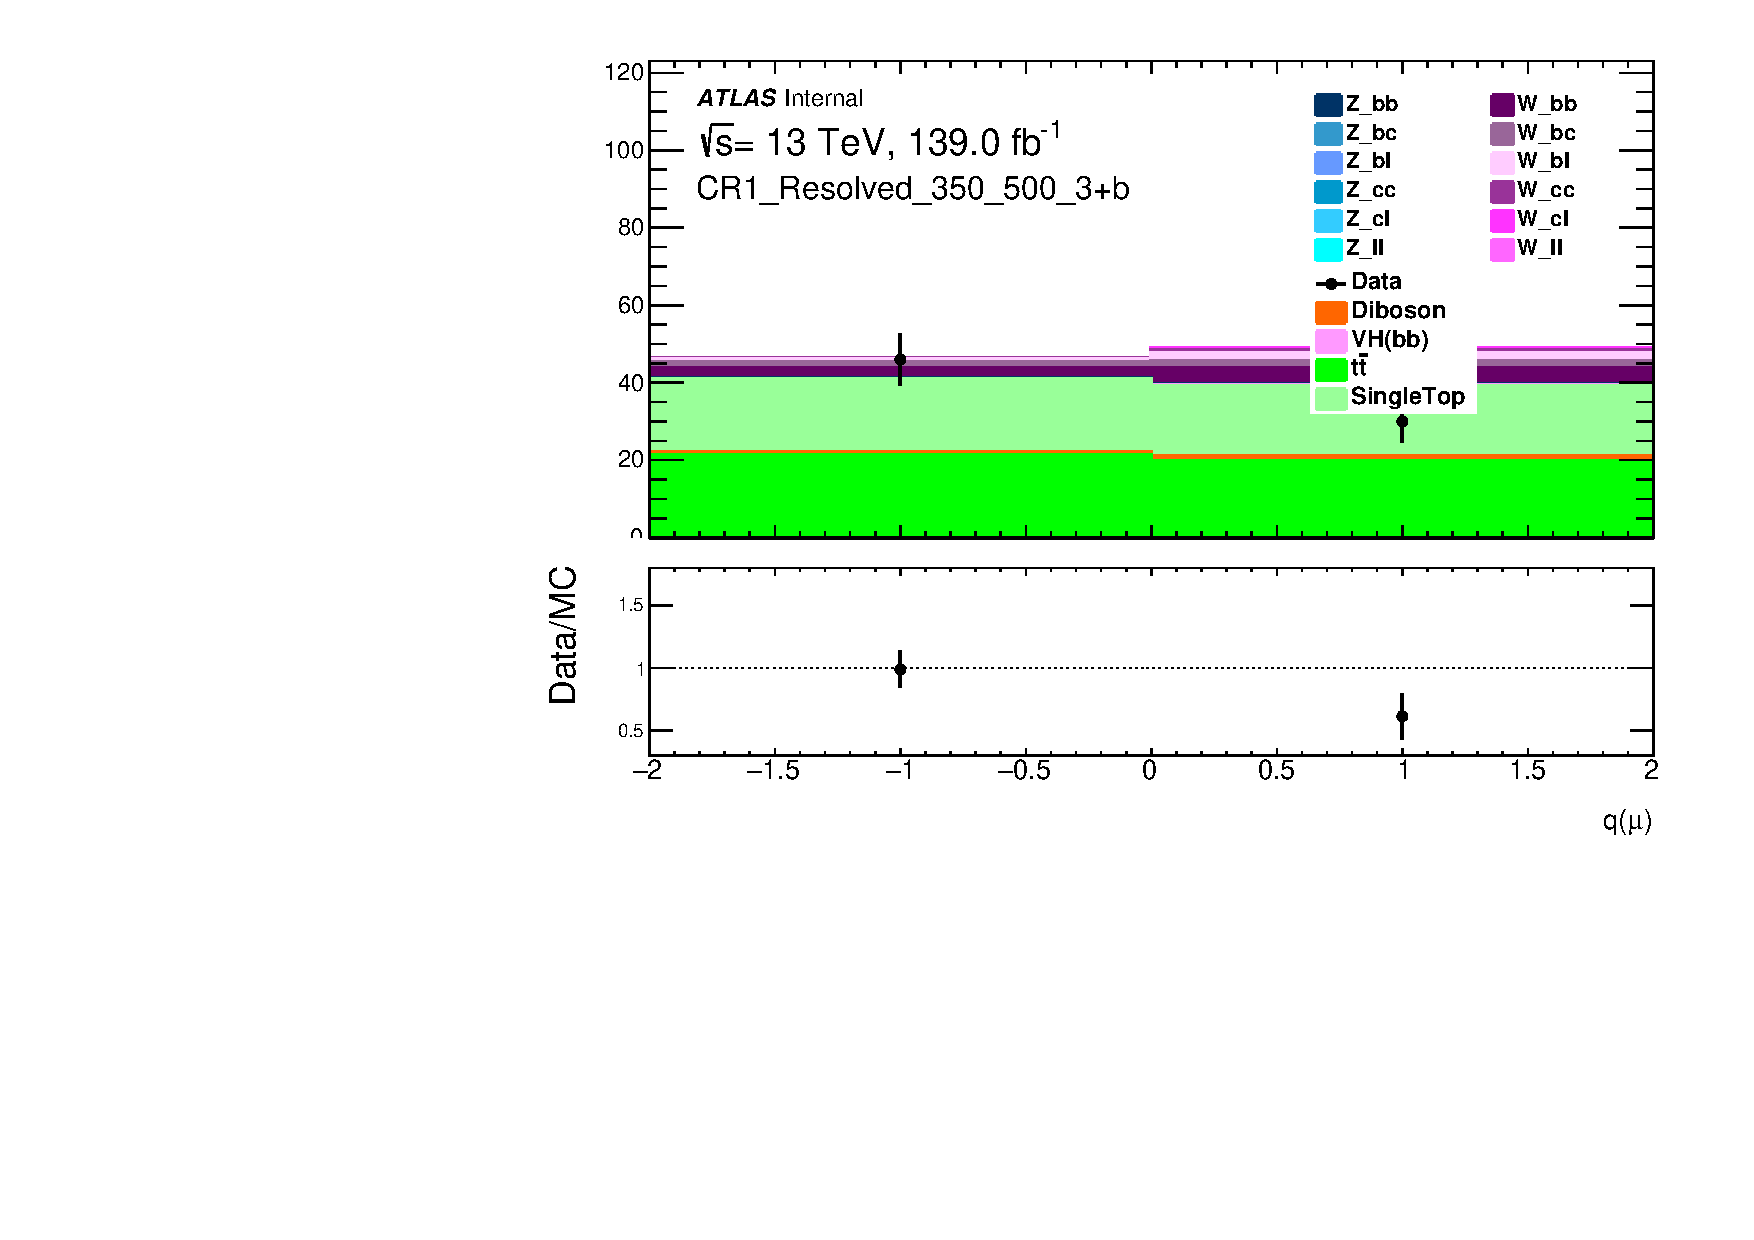
\includegraphics[width=0.46\linewidth]{chapters/c8/figures/1L/DataMC_MonoH_Nominal_CR1_Resolved_350_500_3+b_mu_charge.pdf}
    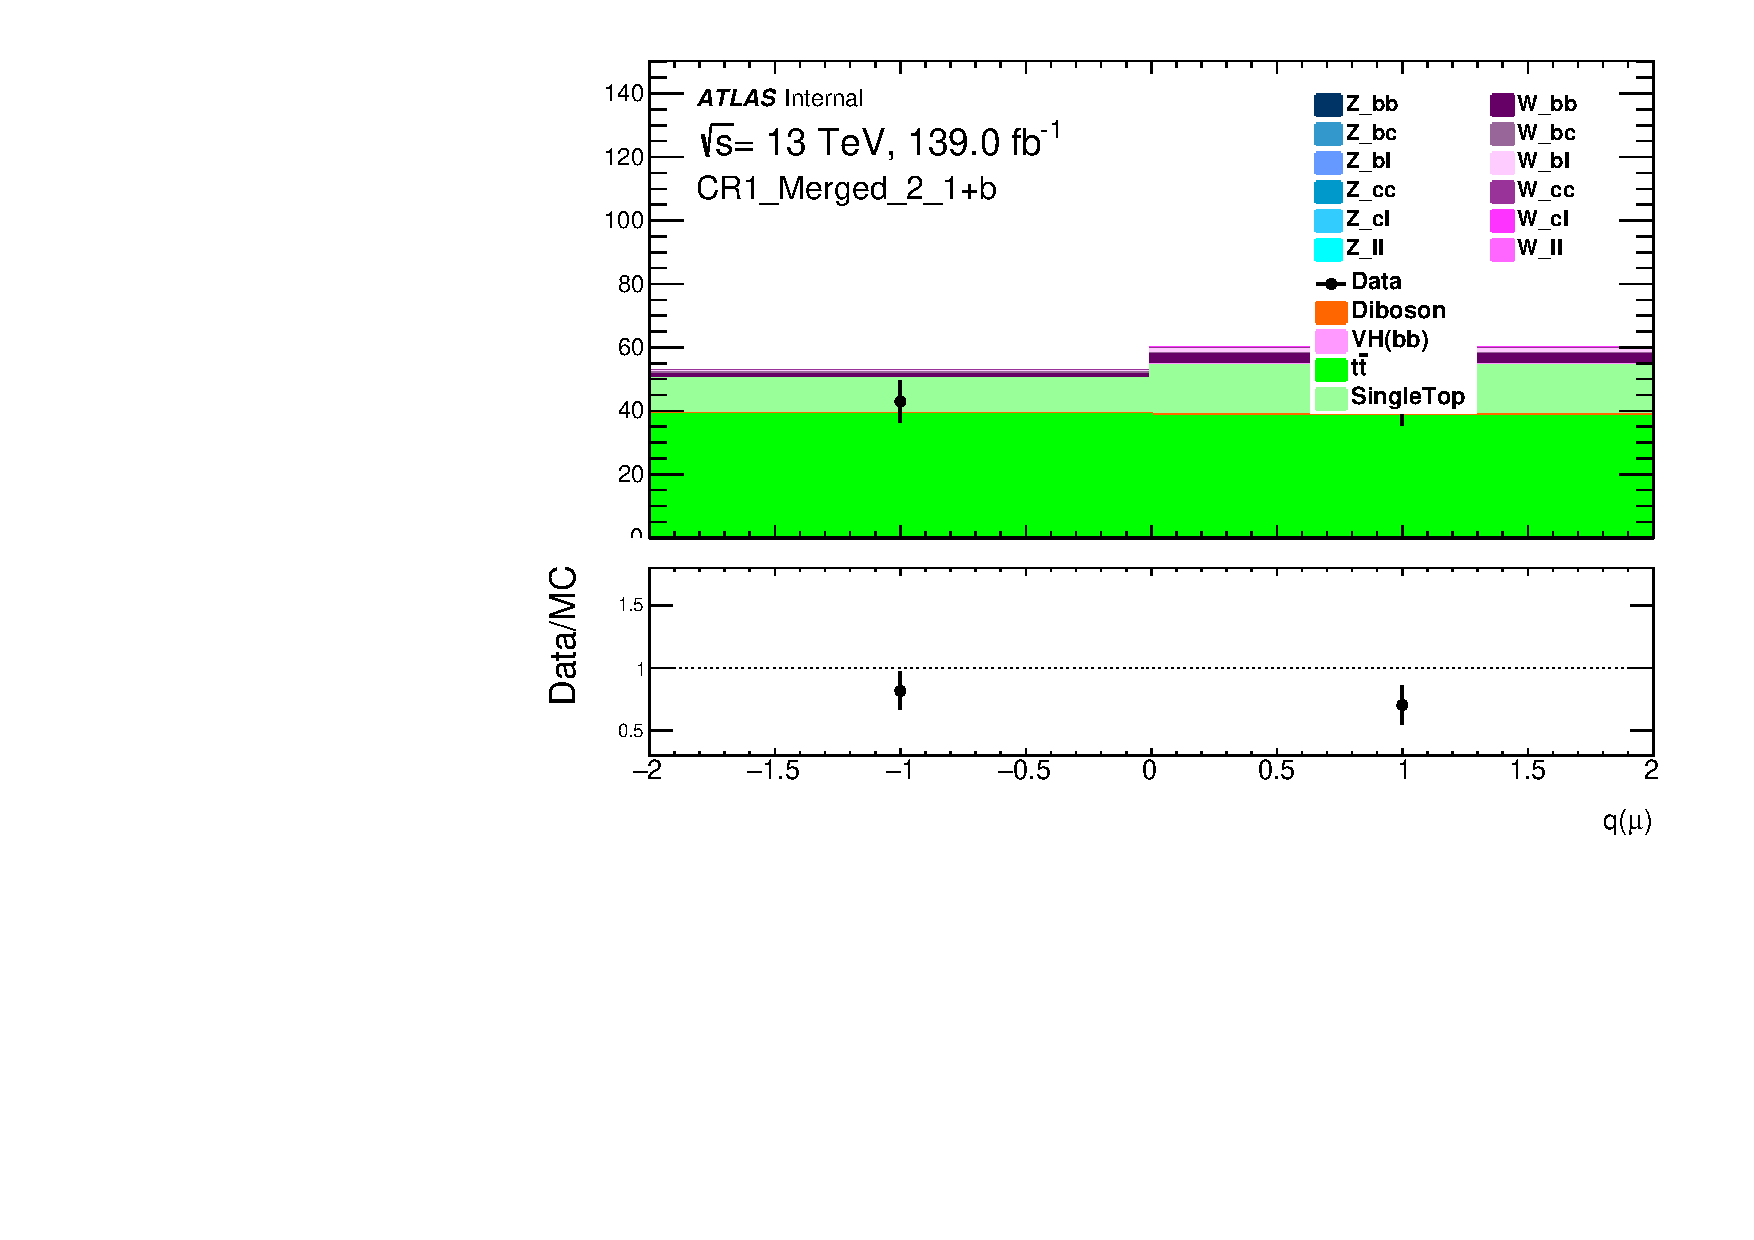
\includegraphics[width=0.46\linewidth]{chapters/c8/figures/1L/DataMC_MonoH_Nominal_CR1_Merged_2_1+b_mu_charge.pdf}
    \caption{Muon charge distribution in the different \met regions with least 3 $b$-tagged jets in the 1-lepton channel.}
    \label{fig:data-mc-1l-mu-charge-3+b}
\end{figure}

\subsection{Control region: 2-lepton}

\begin{figure}[!htb]
    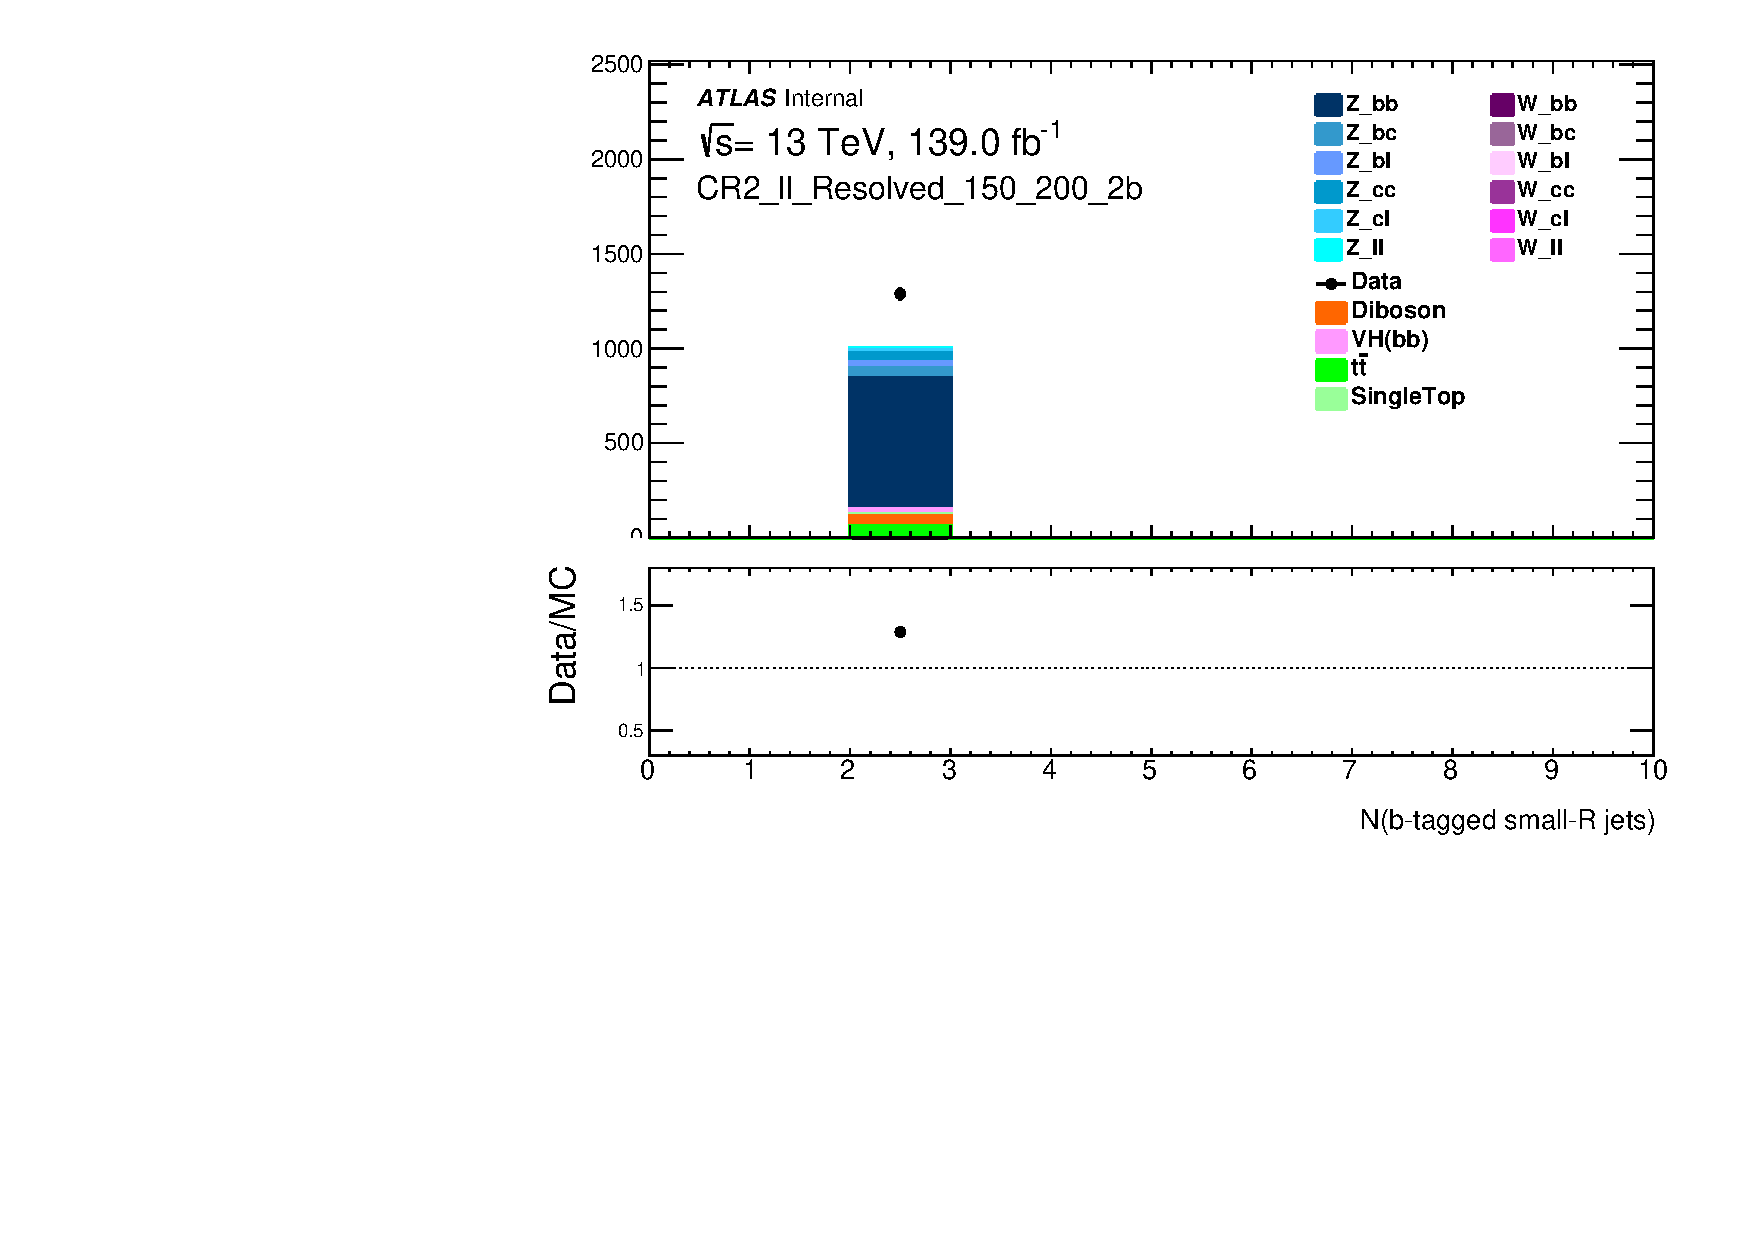
\includegraphics[width=0.46\linewidth]{chapters/c8/figures/2L/DataMC_MonoH_Nominal_CR2_ll_Resolved_150_200_2b_N_BJets_04.pdf}
    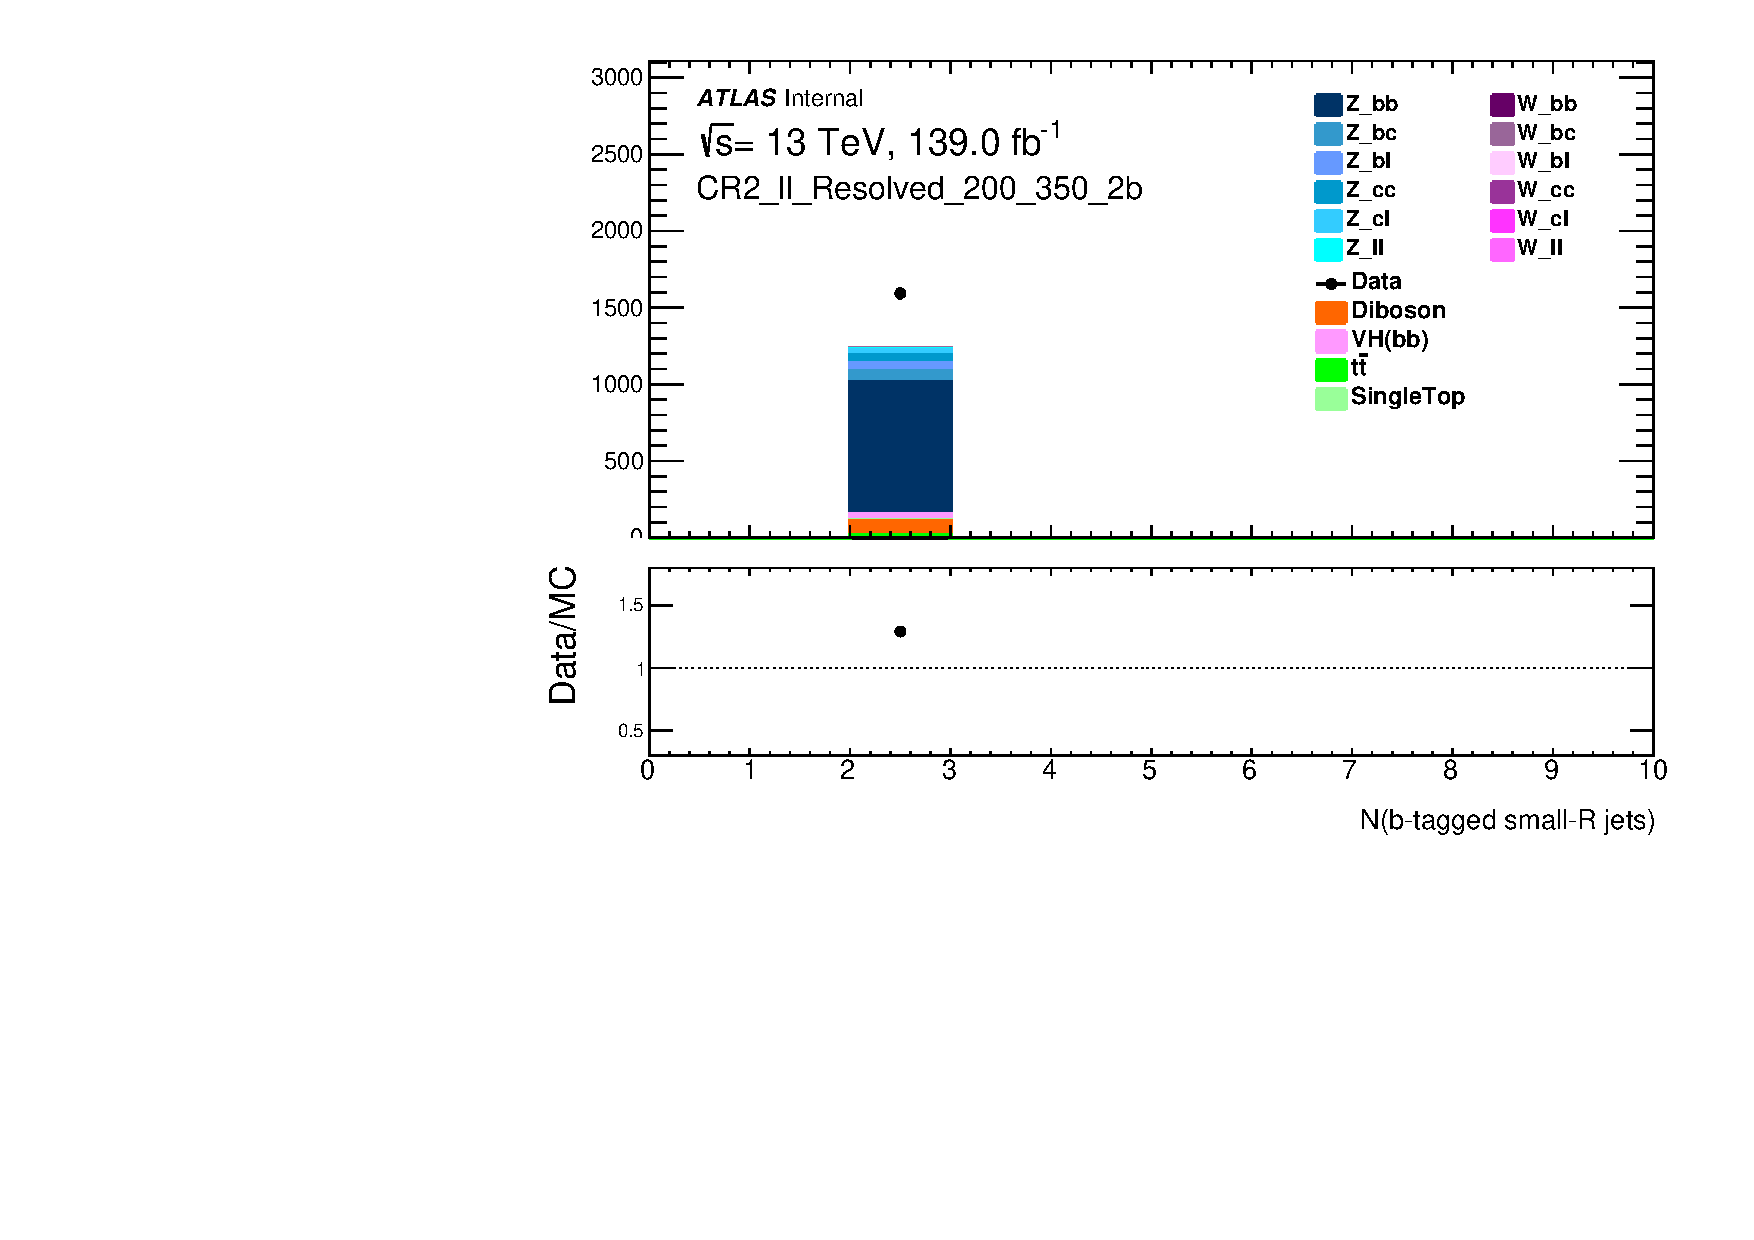
\includegraphics[width=0.46\linewidth]{chapters/c8/figures/2L/DataMC_MonoH_Nominal_CR2_ll_Resolved_200_350_2b_N_BJets_04.pdf}\\
    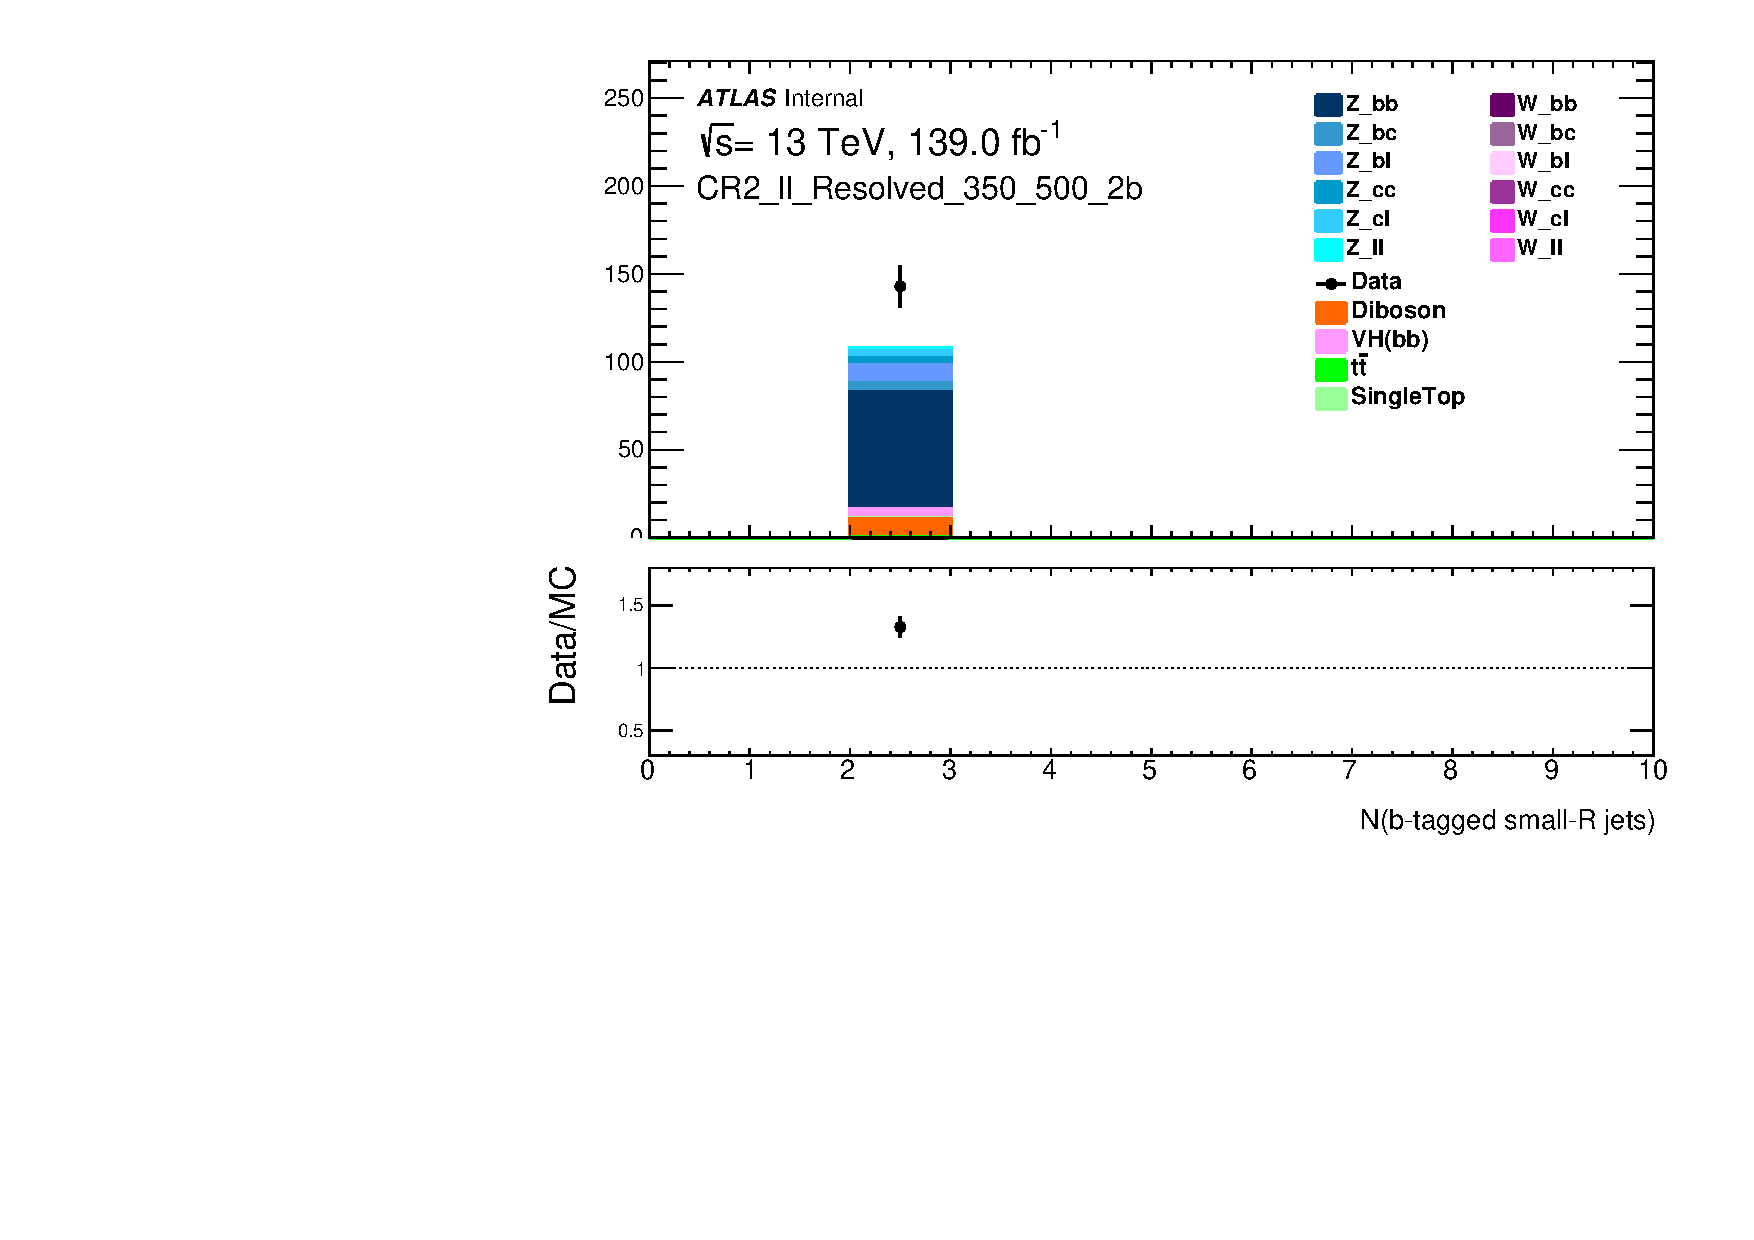
\includegraphics[width=0.46\linewidth]{chapters/c8/figures/2L/DataMC_MonoH_Nominal_CR2_ll_Resolved_350_500_2b_N_BJets_04.pdf}
    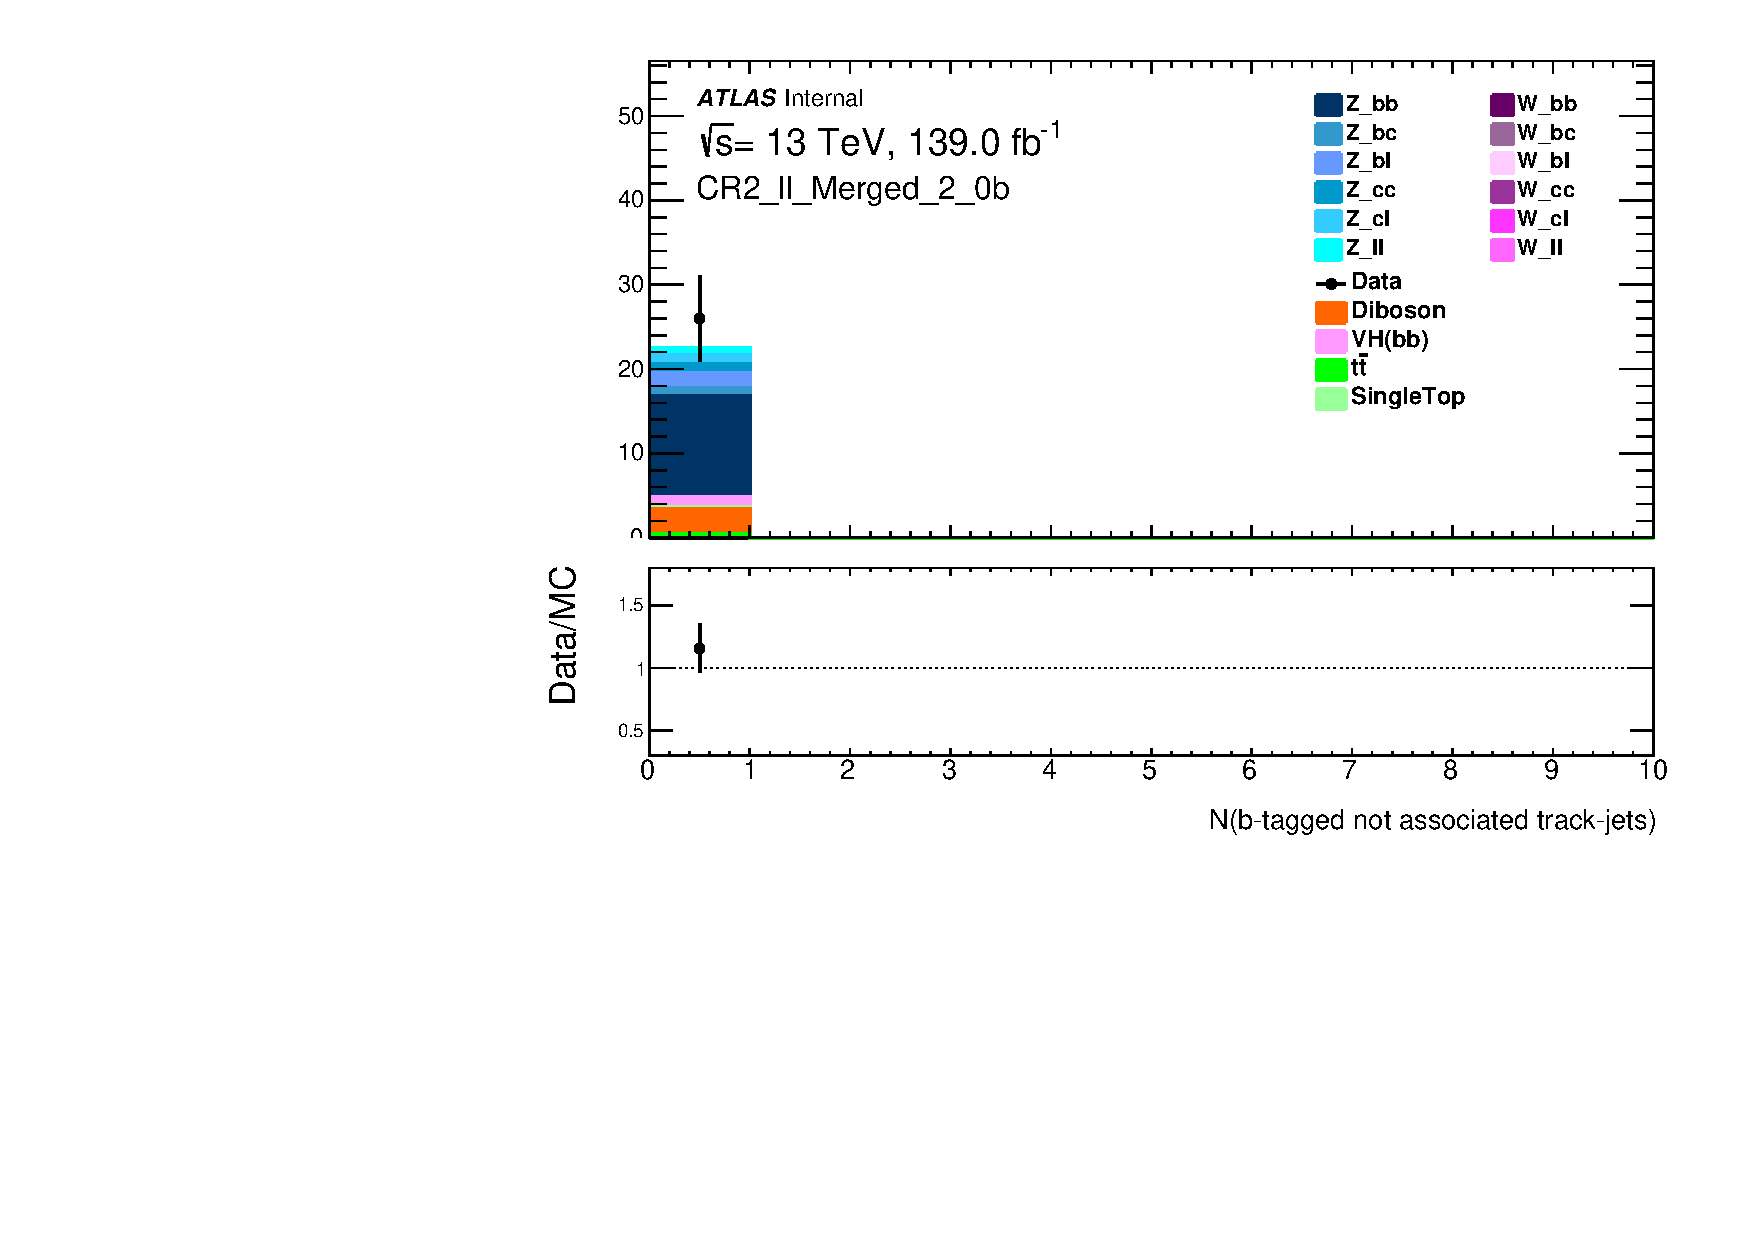
\includegraphics[width=0.46\linewidth]{chapters/c8/figures/2L/DataMC_MonoH_Nominal_CR2_ll_Merged_2_0b_N_BTags_not_associated_02.pdf}
    \caption{Total yields in the 2-lepton control region for different \met regions with 2 $b$-tagged jets.}
    \label{fig:data-mc-2l-ll-mjj-2b}
\end{figure}
  
\begin{figure}[!htb]
    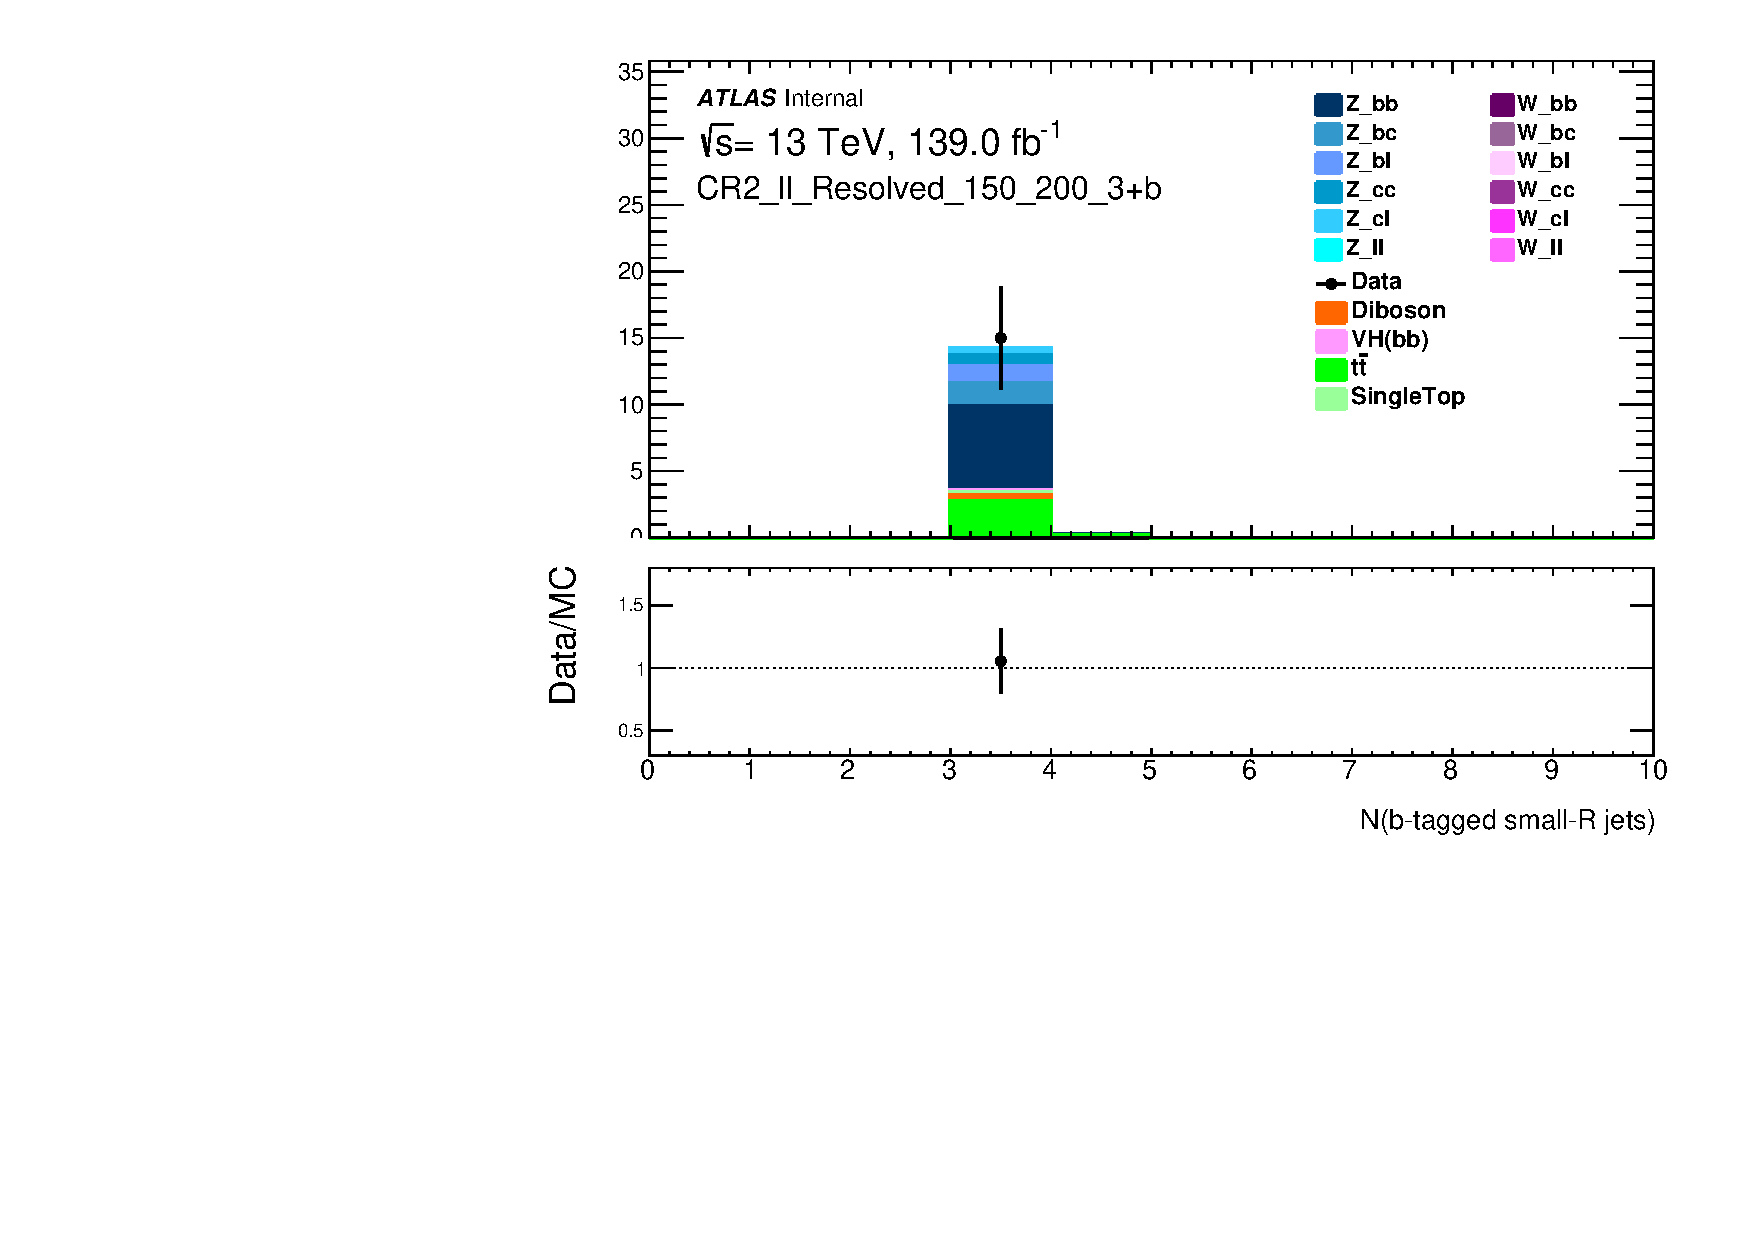
\includegraphics[width=0.46\linewidth]{chapters/c8/figures/2L/DataMC_MonoH_Nominal_CR2_ll_Resolved_150_200_3+b_N_BJets_04.pdf}
    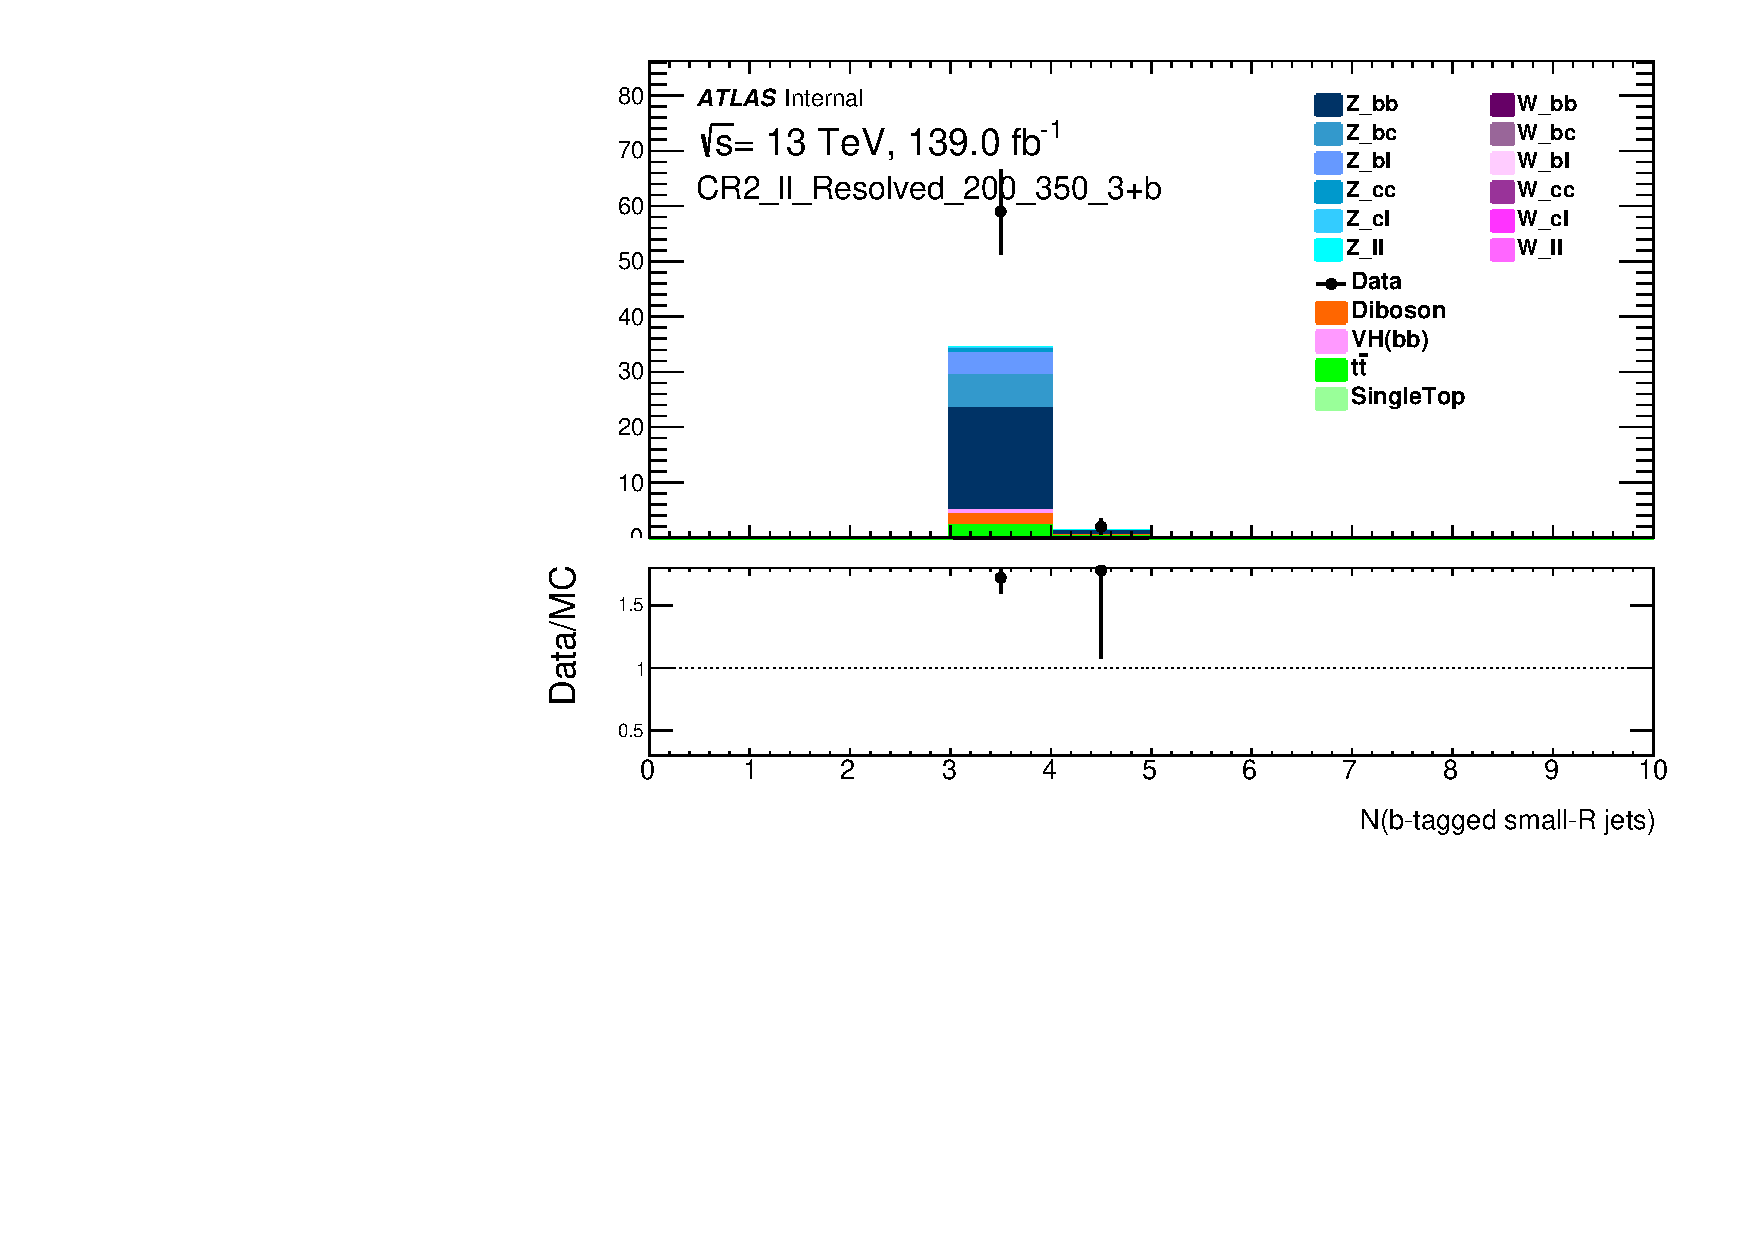
\includegraphics[width=0.46\linewidth]{chapters/c8/figures/2L/DataMC_MonoH_Nominal_CR2_ll_Resolved_200_350_3+b_N_BJets_04.pdf}\\
    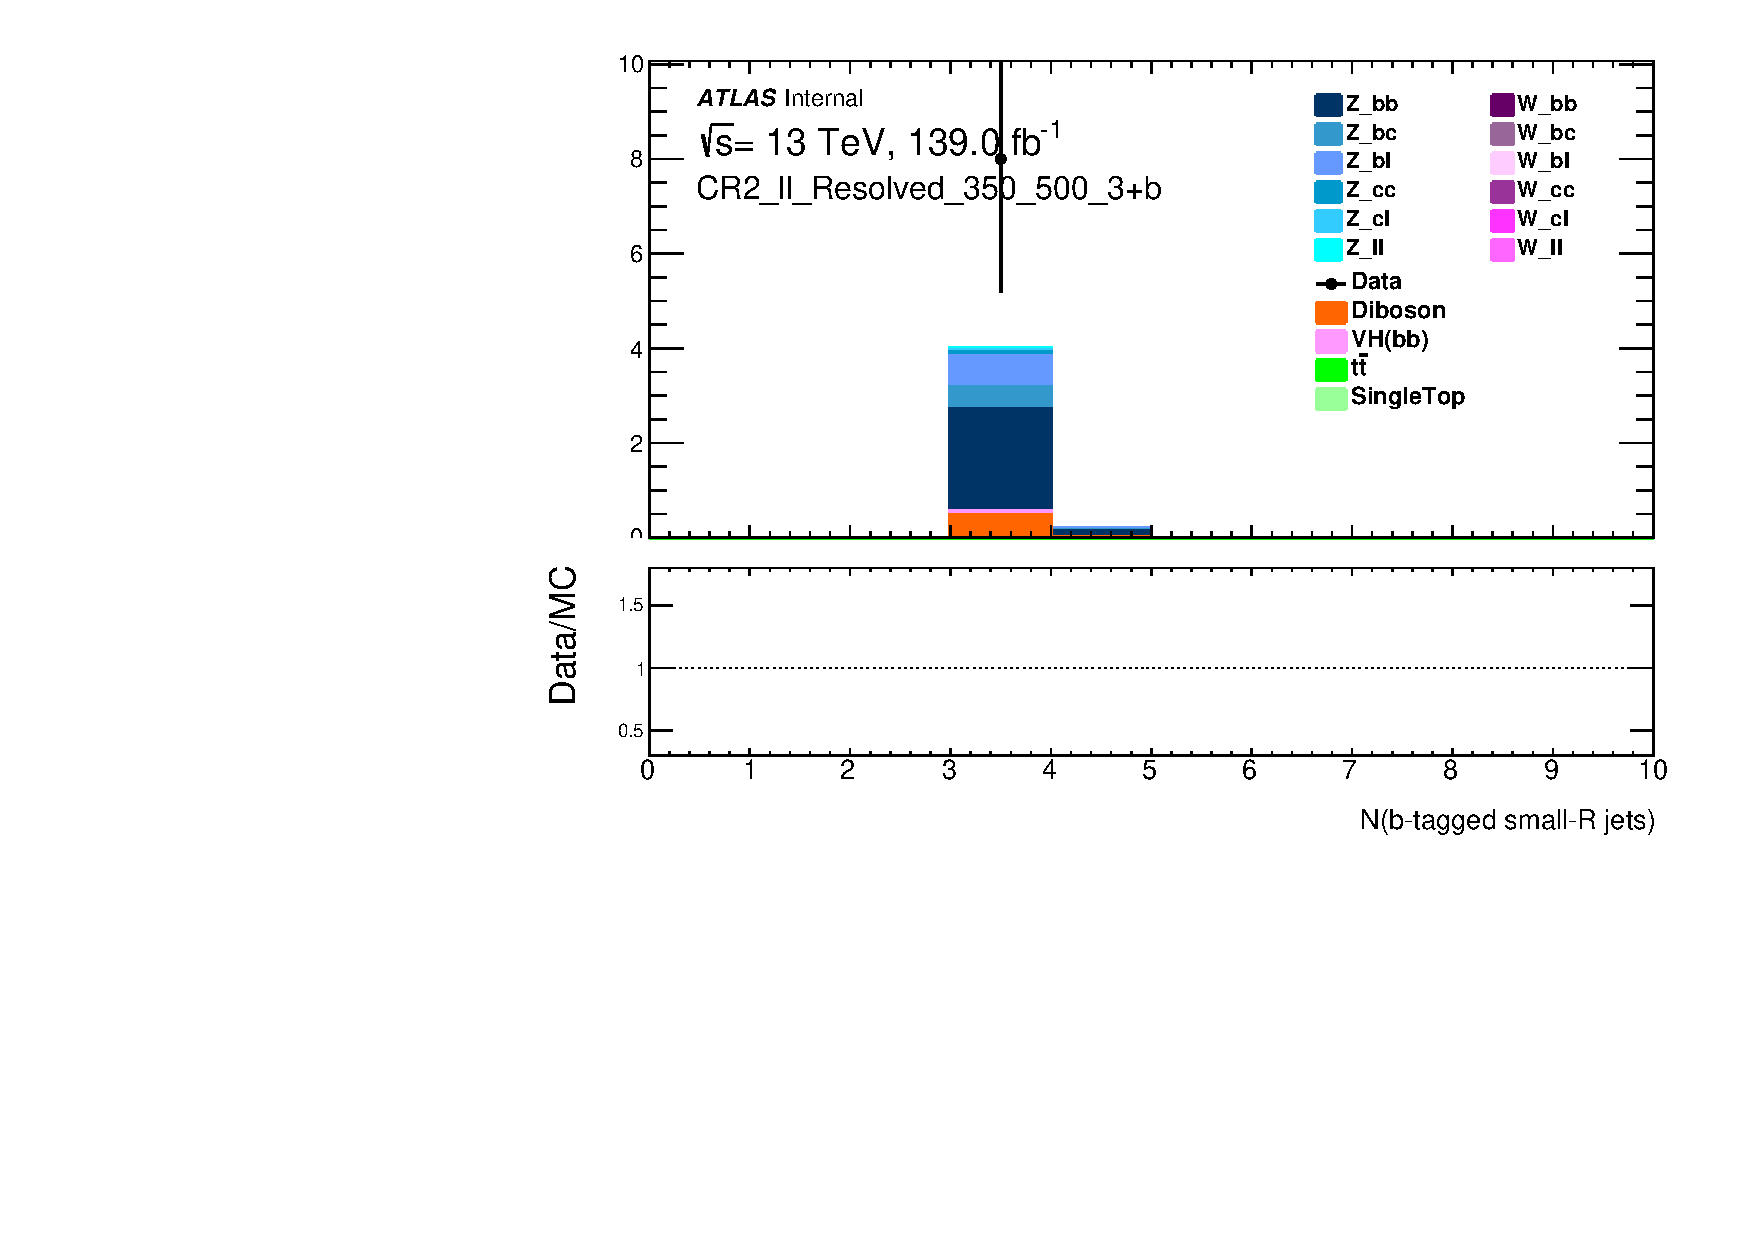
\includegraphics[width=0.46\linewidth]{chapters/c8/figures/2L/DataMC_MonoH_Nominal_CR2_ll_Resolved_350_500_3+b_N_BJets_04.pdf}
    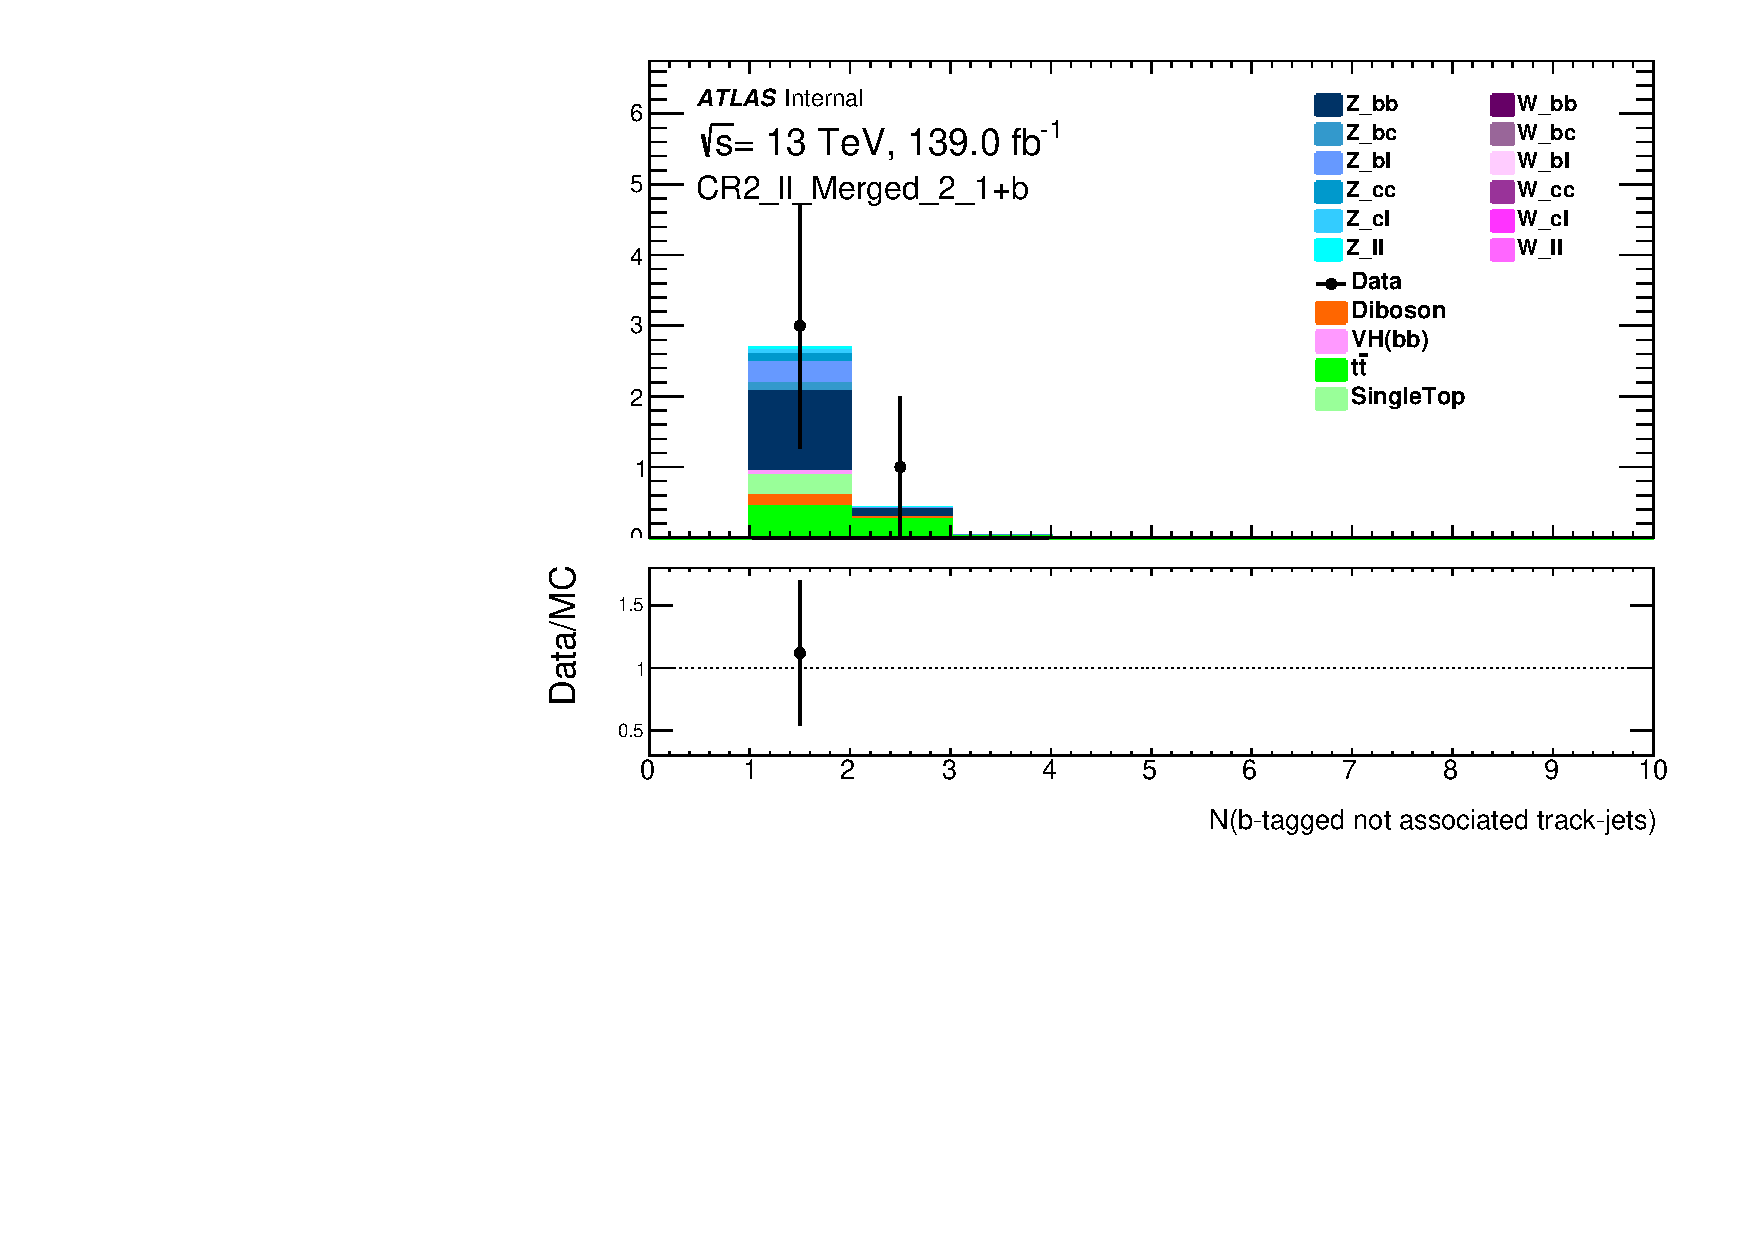
\includegraphics[width=0.46\linewidth]{chapters/c8/figures/2L/DataMC_MonoH_Nominal_CR2_ll_Merged_2_1+b_N_BTags_not_associated_02.pdf}
    \caption{Total yields in the 2-lepton control region for different \met regions with more than 2 $b$-tagged jets.}
    \label{fig:data-mc-2l-ll-mjj-3+b}
\end{figure}
